% Options for packages loaded elsewhere
\PassOptionsToPackage{unicode}{hyperref}
\PassOptionsToPackage{hyphens}{url}
%
\documentclass[
  letterpaper,
]{book}

\usepackage{amsmath,amssymb}
\usepackage{lmodern}
\usepackage{iftex}
\ifPDFTeX
  \usepackage[T1]{fontenc}
  \usepackage[utf8]{inputenc}
  \usepackage{textcomp} % provide euro and other symbols
\else % if luatex or xetex
  \usepackage{unicode-math}
  \defaultfontfeatures{Scale=MatchLowercase}
  \defaultfontfeatures[\rmfamily]{Ligatures=TeX,Scale=1}
\fi
% Use upquote if available, for straight quotes in verbatim environments
\IfFileExists{upquote.sty}{\usepackage{upquote}}{}
\IfFileExists{microtype.sty}{% use microtype if available
  \usepackage[]{microtype}
  \UseMicrotypeSet[protrusion]{basicmath} % disable protrusion for tt fonts
}{}
\makeatletter
\@ifundefined{KOMAClassName}{% if non-KOMA class
  \IfFileExists{parskip.sty}{%
    \usepackage{parskip}
  }{% else
    \setlength{\parindent}{0pt}
    \setlength{\parskip}{6pt plus 2pt minus 1pt}}
}{% if KOMA class
  \KOMAoptions{parskip=half}}
\makeatother
\usepackage{xcolor}
\setlength{\emergencystretch}{3em} % prevent overfull lines
\setcounter{secnumdepth}{5}
% Make \paragraph and \subparagraph free-standing
\ifx\paragraph\undefined\else
  \let\oldparagraph\paragraph
  \renewcommand{\paragraph}[1]{\oldparagraph{#1}\mbox{}}
\fi
\ifx\subparagraph\undefined\else
  \let\oldsubparagraph\subparagraph
  \renewcommand{\subparagraph}[1]{\oldsubparagraph{#1}\mbox{}}
\fi

\usepackage{color}
\usepackage{fancyvrb}
\newcommand{\VerbBar}{|}
\newcommand{\VERB}{\Verb[commandchars=\\\{\}]}
\DefineVerbatimEnvironment{Highlighting}{Verbatim}{commandchars=\\\{\}}
% Add ',fontsize=\small' for more characters per line
\usepackage{framed}
\definecolor{shadecolor}{RGB}{241,243,245}
\newenvironment{Shaded}{\begin{snugshade}}{\end{snugshade}}
\newcommand{\AlertTok}[1]{\textcolor[rgb]{0.68,0.00,0.00}{#1}}
\newcommand{\AnnotationTok}[1]{\textcolor[rgb]{0.37,0.37,0.37}{#1}}
\newcommand{\AttributeTok}[1]{\textcolor[rgb]{0.40,0.45,0.13}{#1}}
\newcommand{\BaseNTok}[1]{\textcolor[rgb]{0.68,0.00,0.00}{#1}}
\newcommand{\BuiltInTok}[1]{\textcolor[rgb]{0.00,0.23,0.31}{#1}}
\newcommand{\CharTok}[1]{\textcolor[rgb]{0.13,0.47,0.30}{#1}}
\newcommand{\CommentTok}[1]{\textcolor[rgb]{0.37,0.37,0.37}{#1}}
\newcommand{\CommentVarTok}[1]{\textcolor[rgb]{0.37,0.37,0.37}{\textit{#1}}}
\newcommand{\ConstantTok}[1]{\textcolor[rgb]{0.56,0.35,0.01}{#1}}
\newcommand{\ControlFlowTok}[1]{\textcolor[rgb]{0.00,0.23,0.31}{#1}}
\newcommand{\DataTypeTok}[1]{\textcolor[rgb]{0.68,0.00,0.00}{#1}}
\newcommand{\DecValTok}[1]{\textcolor[rgb]{0.68,0.00,0.00}{#1}}
\newcommand{\DocumentationTok}[1]{\textcolor[rgb]{0.37,0.37,0.37}{\textit{#1}}}
\newcommand{\ErrorTok}[1]{\textcolor[rgb]{0.68,0.00,0.00}{#1}}
\newcommand{\ExtensionTok}[1]{\textcolor[rgb]{0.00,0.23,0.31}{#1}}
\newcommand{\FloatTok}[1]{\textcolor[rgb]{0.68,0.00,0.00}{#1}}
\newcommand{\FunctionTok}[1]{\textcolor[rgb]{0.28,0.35,0.67}{#1}}
\newcommand{\ImportTok}[1]{\textcolor[rgb]{0.00,0.46,0.62}{#1}}
\newcommand{\InformationTok}[1]{\textcolor[rgb]{0.37,0.37,0.37}{#1}}
\newcommand{\KeywordTok}[1]{\textcolor[rgb]{0.00,0.23,0.31}{#1}}
\newcommand{\NormalTok}[1]{\textcolor[rgb]{0.00,0.23,0.31}{#1}}
\newcommand{\OperatorTok}[1]{\textcolor[rgb]{0.37,0.37,0.37}{#1}}
\newcommand{\OtherTok}[1]{\textcolor[rgb]{0.00,0.23,0.31}{#1}}
\newcommand{\PreprocessorTok}[1]{\textcolor[rgb]{0.68,0.00,0.00}{#1}}
\newcommand{\RegionMarkerTok}[1]{\textcolor[rgb]{0.00,0.23,0.31}{#1}}
\newcommand{\SpecialCharTok}[1]{\textcolor[rgb]{0.37,0.37,0.37}{#1}}
\newcommand{\SpecialStringTok}[1]{\textcolor[rgb]{0.13,0.47,0.30}{#1}}
\newcommand{\StringTok}[1]{\textcolor[rgb]{0.13,0.47,0.30}{#1}}
\newcommand{\VariableTok}[1]{\textcolor[rgb]{0.07,0.07,0.07}{#1}}
\newcommand{\VerbatimStringTok}[1]{\textcolor[rgb]{0.13,0.47,0.30}{#1}}
\newcommand{\WarningTok}[1]{\textcolor[rgb]{0.37,0.37,0.37}{\textit{#1}}}

\providecommand{\tightlist}{%
  \setlength{\itemsep}{0pt}\setlength{\parskip}{0pt}}\usepackage{longtable,booktabs,array}
\usepackage{calc} % for calculating minipage widths
% Correct order of tables after \paragraph or \subparagraph
\usepackage{etoolbox}
\makeatletter
\patchcmd\longtable{\par}{\if@noskipsec\mbox{}\fi\par}{}{}
\makeatother
% Allow footnotes in longtable head/foot
\IfFileExists{footnotehyper.sty}{\usepackage{footnotehyper}}{\usepackage{footnote}}
\makesavenoteenv{longtable}
\usepackage{graphicx}
\makeatletter
\def\maxwidth{\ifdim\Gin@nat@width>\linewidth\linewidth\else\Gin@nat@width\fi}
\def\maxheight{\ifdim\Gin@nat@height>\textheight\textheight\else\Gin@nat@height\fi}
\makeatother
% Scale images if necessary, so that they will not overflow the page
% margins by default, and it is still possible to overwrite the defaults
% using explicit options in \includegraphics[width, height, ...]{}
\setkeys{Gin}{width=\maxwidth,height=\maxheight,keepaspectratio}
% Set default figure placement to htbp
\makeatletter
\def\fps@figure{htbp}
\makeatother
\newlength{\cslhangindent}
\setlength{\cslhangindent}{1.5em}
\newlength{\csllabelwidth}
\setlength{\csllabelwidth}{3em}
\newlength{\cslentryspacingunit} % times entry-spacing
\setlength{\cslentryspacingunit}{\parskip}
\newenvironment{CSLReferences}[2] % #1 hanging-ident, #2 entry spacing
 {% don't indent paragraphs
  \setlength{\parindent}{0pt}
  % turn on hanging indent if param 1 is 1
  \ifodd #1
  \let\oldpar\par
  \def\par{\hangindent=\cslhangindent\oldpar}
  \fi
  % set entry spacing
  \setlength{\parskip}{#2\cslentryspacingunit}
 }%
 {}
\usepackage{calc}
\newcommand{\CSLBlock}[1]{#1\hfill\break}
\newcommand{\CSLLeftMargin}[1]{\parbox[t]{\csllabelwidth}{#1}}
\newcommand{\CSLRightInline}[1]{\parbox[t]{\linewidth - \csllabelwidth}{#1}\break}
\newcommand{\CSLIndent}[1]{\hspace{\cslhangindent}#1}

\makeatletter
\makeatother
\makeatletter
\@ifpackageloaded{bookmark}{}{\usepackage{bookmark}}
\makeatother
\makeatletter
\@ifpackageloaded{caption}{}{\usepackage{caption}}
\AtBeginDocument{%
\ifdefined\contentsname
  \renewcommand*\contentsname{Table of contents}
\else
  \newcommand\contentsname{Table of contents}
\fi
\ifdefined\listfigurename
  \renewcommand*\listfigurename{List of Figures}
\else
  \newcommand\listfigurename{List of Figures}
\fi
\ifdefined\listtablename
  \renewcommand*\listtablename{List of Tables}
\else
  \newcommand\listtablename{List of Tables}
\fi
\ifdefined\figurename
  \renewcommand*\figurename{Figure}
\else
  \newcommand\figurename{Figure}
\fi
\ifdefined\tablename
  \renewcommand*\tablename{Table}
\else
  \newcommand\tablename{Table}
\fi
}
\@ifpackageloaded{float}{}{\usepackage{float}}
\floatstyle{ruled}
\@ifundefined{c@chapter}{\newfloat{codelisting}{h}{lop}}{\newfloat{codelisting}{h}{lop}[chapter]}
\floatname{codelisting}{Listing}
\newcommand*\listoflistings{\listof{codelisting}{List of Listings}}
\makeatother
\makeatletter
\@ifpackageloaded{caption}{}{\usepackage{caption}}
\@ifpackageloaded{subcaption}{}{\usepackage{subcaption}}
\makeatother
\makeatletter
\@ifpackageloaded{tcolorbox}{}{\usepackage[many]{tcolorbox}}
\makeatother
\makeatletter
\@ifundefined{shadecolor}{\definecolor{shadecolor}{rgb}{.97, .97, .97}}
\makeatother
\makeatletter
\makeatother
\ifLuaTeX
  \usepackage{selnolig}  % disable illegal ligatures
\fi
\IfFileExists{bookmark.sty}{\usepackage{bookmark}}{\usepackage{hyperref}}
\IfFileExists{xurl.sty}{\usepackage{xurl}}{} % add URL line breaks if available
\urlstyle{same} % disable monospaced font for URLs
\hypersetup{
  pdftitle={Quantiles, Networks, Time},
  pdfauthor={andrew p blake},
  hidelinks,
  pdfcreator={LaTeX via pandoc}}

\title{Quantiles, Networks, Time}
\author{andrew p blake}
\date{1/1/24}

\begin{document}
\frontmatter
\maketitle
\ifdefined\Shaded\renewenvironment{Shaded}{\begin{tcolorbox}[enhanced, interior hidden, boxrule=0pt, borderline west={3pt}{0pt}{shadecolor}, breakable, sharp corners, frame hidden]}{\end{tcolorbox}}\fi

\renewcommand*\contentsname{Table of contents}
{
\setcounter{tocdepth}{2}
\tableofcontents
}
\mainmatter
\bookmarksetup{startatroot}

\hypertarget{sec-genesis}{%
\chapter*{Genesis}\label{sec-genesis}}
\addcontentsline{toc}{chapter}{Genesis}

\markboth{Genesis}{Genesis}

This book is the result of an initiative the Bank of England began in
the early 1990s, and a prescient one. This was at a major historical
turning point, one that signalled a burgeoning new world order, as the
Iron Curtain crumbled, the European experiment gathered momentum, and
industrial might began an inexorable shift eastwards.

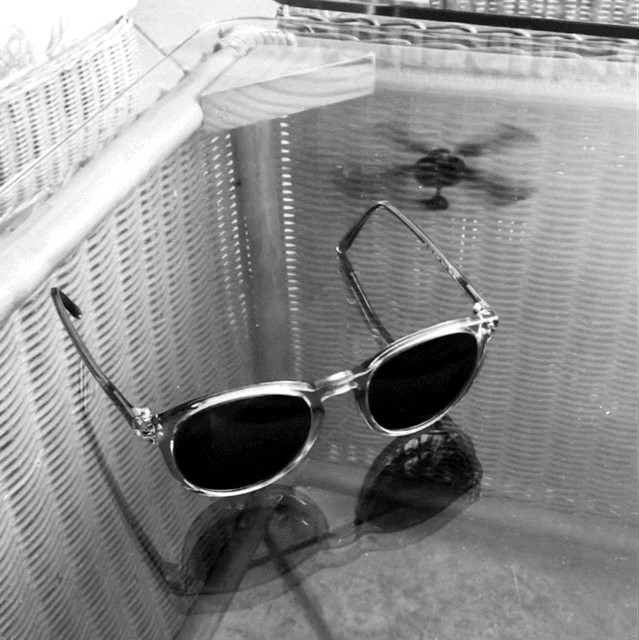
\includegraphics[width=4.375in,height=\textheight]{./Specs.GIF}

Placeholders abound.

\hypertarget{sec-disclaimer}{%
\section*{Disclaimer}\label{sec-disclaimer}}
\addcontentsline{toc}{section}{Disclaimer}

\markright{Disclaimer}

\emph{The Bank of England does not accept any liability for misleading
or inaccurate information or omissions in the information provided. The
subject matter reflects the views of the individual presenter and not
the wider Bank of England or its Policy Committees.}

\part{Introduction}

\hypertarget{introduction-1}{%
\chapter{Introduction}\label{introduction-1}}

This is a book created from markdown and executable code.

See Andrew P. Blake and Mumtaz (2017).

\hypertarget{reading-is-good-for-you}{%
\section{Reading is good for you}\label{reading-is-good-for-you}}

For me, the best (although slightly dated) text is Hastie, Tibshirani,
and Friedman (2009)
\href{https://web.stanford.edu/~hastie/ElemStatLearn/}{The Elements of
Statistical Learning} and the best source for the mathematics, with an
easy-reading version by some of the same authors James et al. (2021)
\href{https://www.statlearning.com/}{Introduction to Statistical
Learning}.

I also rather like Boehmke and Greenwell (2019)
\href{https://bradleyboehmke.github.io/HOML/}{Hands-On Machine Learning
with R} which is something of a cookbook rather than a technical manual
but with wide scope. Taddy (2019) is more elementary.

On text, just read Silge and Robinson (2017)
\href{https://www.tidytextmining.com/}{Text Mining with R: A Tidy
Approach} and then Hvitfeldt and Silge (2021)
\href{https://smltar.com/}{Supervised Machine Learning for Text Analysis
in R}. That's it.

Two books I would solidly recommend to make us all into better
statisticians and not just econometricians are Gelman, Hill, and Vehtari
(2019) \href{http://www.stat.columbia.edu/~gelman/regression}{Regression
and Other Stories}, and McElreath (2020)
\href{https://github.com/rmcelreath/rethinking}{Statistical Rethinking}.

\hypertarget{non-econometric-methods-for-econometricians}{%
\chapter{Non-econometric methods for
econometricians}\label{non-econometric-methods-for-econometricians}}

\hypertarget{selected-ml-and-dataviz-techniques-in-r}{%
\section{Selected ML and Dataviz techniques in
R}\label{selected-ml-and-dataviz-techniques-in-r}}

Econometricians are used to handling data, performing analysis and
reporting results. But somewhere along the line data became big and
unstructured, analysis was now machines learning about something and
outputs became visualisations.

This online seminar takes some big(ish) datasets, sets the machines on
them and draws some great graphs. If you ever wondered what use a tree
was for forecasting or why everything is a network (including neural
ones), or wanted to draw a map with your house in it, or to understand a
document without the bother of reading it (or a few other things
besides) then you might find something to interest you. All done in R.

Specifically, this seminar is designed to introduce some of the key
methods used outside of econometrics that econometricians will find very
useful in their work in a central bank. This includes some important
machine learning techniques as a gateway to others, particularly
tree-based methods and neural networks, as well as text processing and
map making. All the way through there is an emphasis on the network
properties of many of these techniques. We make extensive use of the
\texttt{tidyverse}, including \texttt{ggplot2} and \texttt{tidytext},
and a number of statistics, machine learning, geographical data and
other packages.

The framework for each day is the following:

\begin{itemize}
\tightlist
\item
  Each day is divided into two two-hour sessions starting at 10.30 am
  and 2.00 pm GMT.
\item
  The first hour of each will be an online presentation covering a
  particular topic (or topics) with a look at both techniques and code.
\item
  After a quick break the second hour will be largely devoted to the
  code itself or resources to understand how to code the material.
\end{itemize}

We may run polls during the event to prioritize the topics covered in
the webinars as it is not expected that everyone will be able to try out
everything.

\hypertarget{the-code}{%
\subsection{The code}\label{the-code}}

All code and some of the data will be made available through the Juno
portal. For each presentation the .Rmd (R markdown) file is supplied
that creates the presentation, an HTML file of the presentation for you
to step through which can be re-created from the .Rmd file, and a
further .R file of the code that we use. Some additional code and data
is included, including links to a number of videos that cover some
additional aspects both in this file and in the presentations.

Some data will need to be downloaded from original other sites if all
the examples are to be followed. All code is additionally available at
\url{https://github.com/andrewpeterblake/R2020} or
\url{https://github.com/andrewpeterblake/R2021} or through the QR codes
below.

\begin{figure}

{\centering 
\includegraphics[width=0.33\textwidth,height=\textheight]{./R2021_files/figure-pdf/unnamed-chunk-1-1.pdf}

}

\caption{GitHub: 2020 (grey, left), 2021 (pink, right)}

\end{figure}

\begin{figure}

{\centering 
\includegraphics[width=0.33\textwidth,height=\textheight]{./R2021_files/figure-pdf/unnamed-chunk-1-2.pdf}

}

\caption{GitHub: 2020 (grey, left), 2021 (pink, right)}

\end{figure}

\begin{center}\rule{0.5\linewidth}{0.5pt}\end{center}

\hypertarget{how-to-ensure-rstudio-finds-the-code}{%
\section{HOW TO ENSURE RSTUDIO FINDS THE
CODE}\label{how-to-ensure-rstudio-finds-the-code}}

To use the code, in particular so that R Studio finds the data files
etc, create a directory for each topic, (e.g.~Trees, ANN etc) and copy
the contents from the zip file or GitHub. Then create a new project in R
Studio that uses that directory as its home directory, using ``File/New
Project'' in the drop down menu. Opening files within a project sets the
home directory to that directory, so everything (including the
sub-directories) can be found.

\begin{center}\rule{0.5\linewidth}{0.5pt}\end{center}

\hypertarget{typical-program-structure}{%
\section{Typical program structure}\label{typical-program-structure}}

\hypertarget{day-1-trees-and-maps}{%
\subsection{Day 1: Trees and maps}\label{day-1-trees-and-maps}}

\hypertarget{trees}{%
\subsubsection{Trees}\label{trees}}

\begin{itemize}
\tightlist
\item
  Classification and regression trees
\item
  Econometrics strikes back: Bootstrap/bagging and Boosting/Model
  selection
\item
  Random forests
\item
  Visualising decision trees
\item
  Use example: House prices
\end{itemize}

The presentations for this are \texttt{Trees.html} and
\texttt{LondonHP.html}; The two programs \texttt{TreeCancer.R} and
\texttt{TreeNW.R} are the use examples.

\hypertarget{maps}{%
\subsubsection{Maps}\label{maps}}

\begin{itemize}
\tightlist
\item
  How to draw a map in R
\item
  A guide to some resources
\item
  Choropleths
\item
  Use examples: Climate change, regional data, postcode wrangling
\end{itemize}

The presentation for this is \texttt{MapAER.html} (see also
\texttt{Weatherpretty.html}); The program \texttt{MapAERcode.R} is the
main map drawing code, I've included \texttt{ZAF.R} as as short simple
way and source for two countries, and the directory \texttt{Trendz}
contains the program (\texttt{app.R}) and data for the weather example.

\begin{figure}

\hfill{} 
\includegraphics[width=0.33\textwidth,height=\textheight]{./R2021_files/figure-pdf/unnamed-chunk-2-1.pdf}

\end{figure}

I've included an additional video (red QR code) for more about Shiny.
This uses unemployment data from the
\href{https://www.philadelphiafed.org/surveys-and-data/real-time-data-research/survey-of-professional-forecasters}{Survey
of Professional Forecasters}. The code we look at is for climate change
data \href{https://climateknowledgeportal.worldbank.org/}{World Bank
data}.

A comprehensive treatment of maps is Lovelace, Nowosad, and Muenchow
(2019) \emph{Geocomputation in R}, but it is quite a lot to assimilate
all at once.

\begin{center}\rule{0.5\linewidth}{0.5pt}\end{center}

\hypertarget{day-2-networks}{%
\subsection{Day 2: Networks}\label{day-2-networks}}

\hypertarget{neural-networks}{%
\subsubsection{Neural networks}\label{neural-networks}}

\begin{itemize}
\tightlist
\item
  What is an ANN? Deep learning?
\item
  Function approximation via a network
\item
  Data: fit, validate, test
\item
  Network architecture
\item
  Use examples: House prices revisited
\end{itemize}

The presentation for this is \texttt{IntroANN.html}; The program
\texttt{ANN.R} replicates the ANN estimation. The data used is the same
as for Day 1.

\hypertarget{networks-real-ones}{%
\subsubsection{Networks (real ones)}\label{networks-real-ones}}

\begin{itemize}
\tightlist
\item
  DAGs and ANNs as network graphs
\item
  Incidence matrices
\item
  Measuring connectivity: Degree and betweenness
\item
  Plotting with \texttt{igraph}
\item
  Use examples: Industry inter-relationships
\end{itemize}

\begin{figure}

\hfill{} 
\includegraphics[width=0.25\textwidth,height=\textheight]{./R2021_files/figure-pdf/unnamed-chunk-3-1.pdf}

\end{figure}

\begin{figure}

\hfill{} 
\includegraphics[width=0.25\textwidth,height=\textheight]{./R2021_files/figure-pdf/unnamed-chunk-3-2.pdf}

\end{figure}

The presentation used for the first part of this is \texttt{DAG.html}
and the program \texttt{Draw\_DAG\_ANN.R} draws the ANN examples from
Day 2 Session 1 as well as some of the DAG examples. The example is
modified from Cunningham (2021) \emph{Causal Inference: The Mixtape},
which is a great read with R code. The pdf \texttt{HandShake3.pdf} is
the source of the director network graphs, and \texttt{Graph101a.R} is a
subset of the analytical work on the corruption data set as described in
the post
\href{https://www.r-bloggers.com/2020/01/graph-theory-101-with-corruption-cases-in-spain/}{\emph{Graph
Theory 101}} (purple QR code), which is the work of
\href{https://codingclubuc3m.rbind.io/talk/2020-01-21/}{Marina Medina}
(blue QR code link to presentation site).

\begin{center}\rule{0.5\linewidth}{0.5pt}\end{center}

\hypertarget{day-3-text}{%
\subsection{Day 3: Text}\label{day-3-text}}

\hypertarget{text-modelling-a-tidytext-approach-session-1}{%
\subsubsection{Text modelling, a `tidytext' approach (Session
1)}\label{text-modelling-a-tidytext-approach-session-1}}

\begin{itemize}
\tightlist
\item
  Data cleaning
\item
  Sentiment
\item
  Topic modelling
\end{itemize}

\hypertarget{text-modelling-a-tidytext-approach-session-2}{%
\subsubsection{Text modelling, a `tidytext' approach (Session
2)}\label{text-modelling-a-tidytext-approach-session-2}}

\begin{itemize}
\tightlist
\item
  Parts-of-speech tagging
\item
  Text regression
\item
  Use examples: Central bank minutes, reports
\end{itemize}

\part{Quantiles}

\hypertarget{quantile-regression}{%
\chapter{Quantile regression}\label{quantile-regression}}

This shows how to manipulate data from the SPF in R.

\begin{Shaded}
\begin{Highlighting}[]
\FunctionTok{library}\NormalTok{(readxl)}
\FunctionTok{library}\NormalTok{(xts)}
\FunctionTok{library}\NormalTok{(lubridate)}
\FunctionTok{library}\NormalTok{(tidyverse)}
\FunctionTok{library}\NormalTok{(quantmod)}
\FunctionTok{library}\NormalTok{(quantreg)}
\end{Highlighting}
\end{Shaded}

\hypertarget{getting-the-data}{%
\section{Getting the data}\label{getting-the-data}}

We download the data and save it locally.

\begin{Shaded}
\begin{Highlighting}[]
\NormalTok{h }\OtherTok{\textless{}{-}} \StringTok{"https://www.philadelphiafed.org/{-}/media/frbp/assets/surveys{-}and{-}data/survey{-}of{-}professional{-}forecasters/historical{-}data/"}
\NormalTok{f }\OtherTok{\textless{}{-}} \StringTok{"meanlevel.xlsx"}

\FunctionTok{download.file}\NormalTok{(}\FunctionTok{paste0}\NormalTok{(h, f), }\AttributeTok{destfile=}\NormalTok{f, }\AttributeTok{mode=}\StringTok{"wb"}\NormalTok{)}
\end{Highlighting}
\end{Shaded}

Retrieve the unemployment data for the average unemployment forecast.

\begin{Shaded}
\begin{Highlighting}[]
\NormalTok{UNEMP }\OtherTok{\textless{}{-}}\NormalTok{ f }\SpecialCharTok{\%\textgreater{}\%}
  \FunctionTok{read\_excel}\NormalTok{(}\AttributeTok{na=}\StringTok{"\#N/A"}\NormalTok{, }\AttributeTok{sheet=}\StringTok{"UNEMP"}\NormalTok{) }\SpecialCharTok{\%\textgreater{}\%} 
  \FunctionTok{mutate}\NormalTok{(}\AttributeTok{Date=}\FunctionTok{as.Date}\NormalTok{(}\FunctionTok{as.yearqtr}\NormalTok{(}\FunctionTok{paste}\NormalTok{(YEAR, QUARTER), }\AttributeTok{format=}\StringTok{"\%Y \%q"}\NormalTok{))) }

\NormalTok{Usel }\OtherTok{\textless{}{-}}\NormalTok{ UNEMP }\SpecialCharTok{\%\textgreater{}\%} 
  \FunctionTok{select}\NormalTok{(Date, UNEMP1, UNEMP3, UNEMP4, UNEMP5, UNEMP6) }\SpecialCharTok{\%\textgreater{}\%}
  \FunctionTok{mutate}\NormalTok{(}\AttributeTok{UNRATE =} \FunctionTok{lead}\NormalTok{(UNEMP1,}\DecValTok{1}\NormalTok{)) }\SpecialCharTok{\%\textgreater{}\%}
  \FunctionTok{select}\NormalTok{(Date, UNRATE, }
         \AttributeTok{UNEMP1=}\NormalTok{UNEMP3, }\AttributeTok{UNEMP2=}\NormalTok{UNEMP4, }\AttributeTok{UNEMP3=}\NormalTok{UNEMP5, }\AttributeTok{UNEMP4=}\NormalTok{UNEMP6) }\SpecialCharTok{\%\textgreater{}\%}
  \FunctionTok{mutate}\NormalTok{(}\AttributeTok{UNEMP1 =} \FunctionTok{lag}\NormalTok{(UNEMP1,}\DecValTok{1}\NormalTok{), }
         \AttributeTok{UNEMP2 =} \FunctionTok{lag}\NormalTok{(UNEMP2,}\DecValTok{2}\NormalTok{), }
         \AttributeTok{UNEMP3 =} \FunctionTok{lag}\NormalTok{(UNEMP3,}\DecValTok{3}\NormalTok{), }
         \AttributeTok{UNEMP4 =} \FunctionTok{lag}\NormalTok{(UNEMP4,}\DecValTok{4}\NormalTok{)) }\SpecialCharTok{\%\textgreater{}\%}
  \FunctionTok{pivot\_longer}\NormalTok{(}\AttributeTok{cols =} \SpecialCharTok{{-}}\FunctionTok{c}\NormalTok{(Date, UNRATE), }\AttributeTok{names\_to=}\StringTok{"Which"}\NormalTok{, }\AttributeTok{values\_to=}\StringTok{"Val"}\NormalTok{) }\SpecialCharTok{\%\textgreater{}\%}
  \FunctionTok{filter}\NormalTok{(}\FunctionTok{year}\NormalTok{(Date) }\SpecialCharTok{\textgreater{}} \DecValTok{2000}\NormalTok{)}
\end{Highlighting}
\end{Shaded}

\hypertarget{plots}{%
\section{Plots}\label{plots}}

\begin{Shaded}
\begin{Highlighting}[]
\NormalTok{Usel }\SpecialCharTok{\%\textgreater{}\%} 
  \FunctionTok{ggplot}\NormalTok{(}\FunctionTok{aes}\NormalTok{(}\AttributeTok{x=}\NormalTok{Date)) }\SpecialCharTok{+} 
  \FunctionTok{geom\_line}\NormalTok{(}\FunctionTok{aes}\NormalTok{(}\AttributeTok{y=}\NormalTok{UNRATE), }\AttributeTok{colour=}\StringTok{"red"}\NormalTok{) }\SpecialCharTok{+} 
  \FunctionTok{geom\_point}\NormalTok{(}\FunctionTok{aes}\NormalTok{(}\AttributeTok{y=}\NormalTok{Val, }\AttributeTok{colour=}\NormalTok{Which, }\AttributeTok{shape=}\NormalTok{Which)) }\SpecialCharTok{+}
  \FunctionTok{theme\_light}\NormalTok{() }\SpecialCharTok{+} 
  \FunctionTok{labs}\NormalTok{(}\AttributeTok{title=}\StringTok{"Mean unemployment forecasts"}\NormalTok{, }\AttributeTok{x=}\StringTok{""}\NormalTok{, }\AttributeTok{y=}\StringTok{""}\NormalTok{, }\AttributeTok{caption=}\StringTok{"Source: SPF"}\NormalTok{)}
\end{Highlighting}
\end{Shaded}

\begin{figure}[H]

{\centering 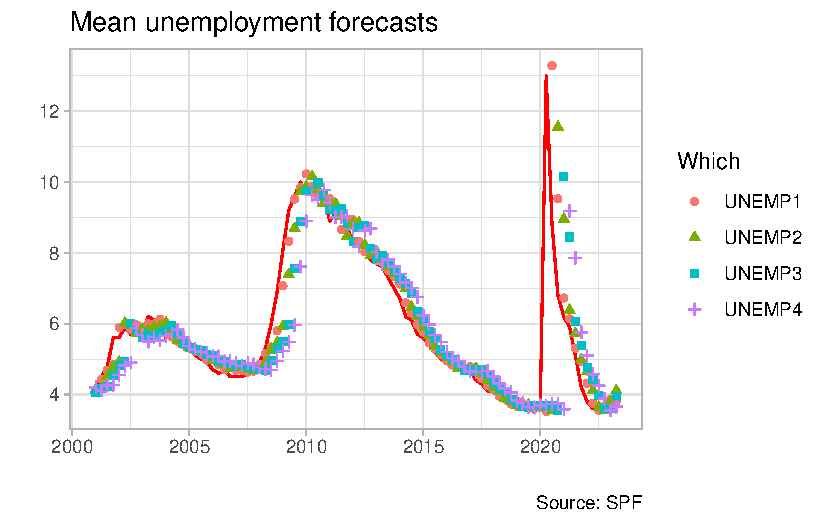
\includegraphics{./QR_files/figure-pdf/unnamed-chunk-2-1.pdf}

}

\end{figure}

\part{Networks}

\hypertarget{causal-inference}{%
\chapter{Causal Inference}\label{causal-inference}}

Outline how to solve the Pearl, Glymour, and Jewell (2016) exercises in
R.

\hypertarget{study-question-1.3.2}{%
\section{Study question 1.3.2}\label{study-question-1.3.2}}

Data:

\begin{Shaded}
\begin{Highlighting}[]
\FunctionTok{library}\NormalTok{(tidyverse)}
\NormalTok{ed }\OtherTok{\textless{}{-}} \FunctionTok{tibble}\NormalTok{(}\AttributeTok{Gender =} \FunctionTok{c}\NormalTok{(}\StringTok{"M"}\NormalTok{,}\StringTok{"M"}\NormalTok{,}\StringTok{"M"}\NormalTok{,}\StringTok{"M"}\NormalTok{,}\StringTok{"F"}\NormalTok{,}\StringTok{"F"}\NormalTok{,}\StringTok{"F"}\NormalTok{,}\StringTok{"F"}\NormalTok{),}
             \AttributeTok{eLevel =} \FunctionTok{c}\NormalTok{(}\StringTok{"U"}\NormalTok{,}\StringTok{"H"}\NormalTok{,}\StringTok{"C"}\NormalTok{,}\StringTok{"G"}\NormalTok{,}\StringTok{"U"}\NormalTok{,}\StringTok{"H"}\NormalTok{,}\StringTok{"C"}\NormalTok{,}\StringTok{"G"}\NormalTok{),}
             \AttributeTok{num    =} \FunctionTok{c}\NormalTok{(}\DecValTok{112}\NormalTok{,}\DecValTok{231}\NormalTok{,}\DecValTok{595}\NormalTok{,}\DecValTok{242}\NormalTok{,}\DecValTok{136}\NormalTok{,}\DecValTok{189}\NormalTok{,}\DecValTok{763}\NormalTok{,}\DecValTok{172}\NormalTok{)) }\SpecialCharTok{\%\textgreater{}\%}
  \FunctionTok{mutate}\NormalTok{(}\AttributeTok{total =} \FunctionTok{sum}\NormalTok{(num))}
\end{Highlighting}
\end{Shaded}

which we tabulate as

\begin{Shaded}
\begin{Highlighting}[]
\NormalTok{ed }\SpecialCharTok{\%\textgreater{}\%}
  \FunctionTok{kable}\NormalTok{()}
\end{Highlighting}
\end{Shaded}

\begin{longtable}[]{@{}llrr@{}}
\toprule()
Gender & eLevel & num & total \\
\midrule()
\endhead
M & U & 112 & 2440 \\
M & H & 231 & 2440 \\
M & C & 595 & 2440 \\
M & G & 242 & 2440 \\
F & U & 136 & 2440 \\
F & H & 189 & 2440 \\
F & C & 763 & 2440 \\
F & G & 172 & 2440 \\
\bottomrule()
\end{longtable}

\hypertarget{exercises-and-answers}{%
\section{Exercises and answers}\label{exercises-and-answers}}

\hypertarget{find-pelevel-h}{%
\subsection{\texorpdfstring{Find
\(P(eLevel = H)\)}{Find P(eLevel = H)}}\label{find-pelevel-h}}

\begin{Shaded}
\begin{Highlighting}[]
\NormalTok{ed }\SpecialCharTok{\%\textgreater{}\%}
  \FunctionTok{filter}\NormalTok{(eLevel }\SpecialCharTok{==} \StringTok{"H"}\NormalTok{) }\SpecialCharTok{\%\textgreater{}\%}
  \FunctionTok{mutate}\NormalTok{(}\AttributeTok{p\_H =} \FunctionTok{sum}\NormalTok{(num)}\SpecialCharTok{/}\NormalTok{total) }\SpecialCharTok{\%\textgreater{}\%}
  \FunctionTok{kable}\NormalTok{()}
\end{Highlighting}
\end{Shaded}

\begin{longtable}[]{@{}llrrr@{}}
\toprule()
Gender & eLevel & num & total & p\_H \\
\midrule()
\endhead
M & H & 231 & 2440 & 0.1721311 \\
F & H & 189 & 2440 & 0.1721311 \\
\bottomrule()
\end{longtable}

\hypertarget{find-pelevel-h-vee-gender-f}{%
\subsection{\texorpdfstring{Find
\(P(eLevel = H\ \vee \ Gender = F)\)}{Find P(eLevel = H\textbackslash{} \textbackslash vee \textbackslash{} Gender = F)}}\label{find-pelevel-h-vee-gender-f}}

\begin{Shaded}
\begin{Highlighting}[]
\NormalTok{ed }\SpecialCharTok{\%\textgreater{}\%}
  \FunctionTok{filter}\NormalTok{(Gender }\SpecialCharTok{==} \StringTok{"F"} \SpecialCharTok{|}\NormalTok{ eLevel }\SpecialCharTok{==} \StringTok{"H"}\NormalTok{) }\SpecialCharTok{\%\textgreater{}\%}
  \FunctionTok{mutate}\NormalTok{(}\AttributeTok{p\_HorF =} \FunctionTok{sum}\NormalTok{(num)}\SpecialCharTok{/}\NormalTok{total) }\SpecialCharTok{\%\textgreater{}\%}
  \FunctionTok{kable}\NormalTok{()}
\end{Highlighting}
\end{Shaded}

\begin{longtable}[]{@{}llrrr@{}}
\toprule()
Gender & eLevel & num & total & p\_HorF \\
\midrule()
\endhead
M & H & 231 & 2440 & 0.6110656 \\
F & U & 136 & 2440 & 0.6110656 \\
F & H & 189 & 2440 & 0.6110656 \\
F & C & 763 & 2440 & 0.6110656 \\
F & G & 172 & 2440 & 0.6110656 \\
\bottomrule()
\end{longtable}

\hypertarget{find-pelevel-h-gender-f}{%
\subsection{\texorpdfstring{Find
\(P(eLevel = H\ |\ Gender = F)\)}{Find P(eLevel = H\textbackslash{} \textbar\textbackslash{} Gender = F)}}\label{find-pelevel-h-gender-f}}

\begin{Shaded}
\begin{Highlighting}[]
\NormalTok{ed }\SpecialCharTok{\%\textgreater{}\%}
  \FunctionTok{filter}\NormalTok{(Gender }\SpecialCharTok{==} \StringTok{"F"}\NormalTok{) }\SpecialCharTok{\%\textgreater{}\%}
  \FunctionTok{mutate}\NormalTok{(}\AttributeTok{tcond =} \FunctionTok{sum}\NormalTok{(num)) }\SpecialCharTok{\%\textgreater{}\%} 
  \FunctionTok{filter}\NormalTok{(eLevel }\SpecialCharTok{==} \StringTok{"H"}\NormalTok{) }\SpecialCharTok{\%\textgreater{}\%}
  \FunctionTok{mutate}\NormalTok{(}\AttributeTok{p\_HgivenF =} \FunctionTok{sum}\NormalTok{(num)}\SpecialCharTok{/}\NormalTok{tcond) }\SpecialCharTok{\%\textgreater{}\%}
  \FunctionTok{kable}\NormalTok{()}
\end{Highlighting}
\end{Shaded}

\begin{longtable}[]{@{}llrrrr@{}}
\toprule()
Gender & eLevel & num & total & tcond & p\_HgivenF \\
\midrule()
\endhead
F & H & 189 & 2440 & 1260 & 0.15 \\
\bottomrule()
\end{longtable}

\hypertarget{find-pgender-f-elevel-h}{%
\subsection{\texorpdfstring{Find
\(P(Gender = F\ | \ eLevel = H)\)}{Find P(Gender = F\textbackslash{} \textbar{} \textbackslash{} eLevel = H)}}\label{find-pgender-f-elevel-h}}

\begin{Shaded}
\begin{Highlighting}[]
\NormalTok{ed }\SpecialCharTok{\%\textgreater{}\%}
  \FunctionTok{filter}\NormalTok{(eLevel }\SpecialCharTok{==} \StringTok{"H"}\NormalTok{) }\SpecialCharTok{\%\textgreater{}\%}
  \FunctionTok{mutate}\NormalTok{(}\AttributeTok{tcond =} \FunctionTok{sum}\NormalTok{(num)) }\SpecialCharTok{\%\textgreater{}\%} 
  \FunctionTok{filter}\NormalTok{(Gender }\SpecialCharTok{==} \StringTok{"F"}\NormalTok{) }\SpecialCharTok{\%\textgreater{}\%}
  \FunctionTok{mutate}\NormalTok{(}\AttributeTok{p\_FgivenH =} \FunctionTok{sum}\NormalTok{(num)}\SpecialCharTok{/}\NormalTok{tcond) }\SpecialCharTok{\%\textgreater{}\%}
  \FunctionTok{kable}\NormalTok{()}
\end{Highlighting}
\end{Shaded}

\begin{longtable}[]{@{}llrrrr@{}}
\toprule()
Gender & eLevel & num & total & tcond & p\_FgivenH \\
\midrule()
\endhead
F & H & 189 & 2440 & 420 & 0.45 \\
\bottomrule()
\end{longtable}

\hypertarget{mapping-regional-house-price-inflation}{%
\chapter{Mapping regional house price
inflation}\label{mapping-regional-house-price-inflation}}

\hypertarget{how-heterogenous-is-uk-house-price-inflation}{%
\section{How heterogenous is UK house price
inflation?}\label{how-heterogenous-is-uk-house-price-inflation}}

A simple enough question, and one that Bahaj, Foulis, and Pinter (2020)
thought was best answered with a map -- actually a referee asked for
one. As I know how to draw a map in R they asked me if I could do it.
Well yes, but there are some particular difficulties.

\begin{itemize}
\tightlist
\item
  The UK (actually Great Britain) is an awkward (but not too awkward)
  shape.
\item
  Population in the UK is heavily concentrated in a small number of
  centres, such as London or Manchester.
\item
  There are three different periods to compare.
\item
  It has to be in grayscale.
\end{itemize}

Before all of this we need some data, with boundaries that correspond to
areas that we have data for. The regional inflation data is available at
the level of the
\href{https://www.gov.uk/government/organisations/land-registry}{Land
Registry}, which almost by local authority but amalgamates a number of
the areas. So a map at Local Authority level would be fine as long as we
can amalgamate some of the regions.

The map data used here is available from the UK's
\href{https://geoportal.statistics.gov.uk/}{ONS geoportal}, with a lot
of administrative data available including local authority boundaries.
The Local Authority data is specifically available from
\href{https://geoportal.statistics.gov.uk/maps/lad-dec-2015-generalised-clipped-boundaries-gb}{here},
where I use the clipped full extent version. There are a number of
possibilities, but in general high water mark, and enough but not too
much detail is needed.

\begin{Shaded}
\begin{Highlighting}[]
\FunctionTok{library}\NormalTok{(tidyverse)}
\FunctionTok{library}\NormalTok{(readxl)}
\FunctionTok{library}\NormalTok{(sf)}
\end{Highlighting}
\end{Shaded}

The information in the map file is comprehensive, and by Local Authority
as of December 2015.

\begin{Shaded}
\begin{Highlighting}[]
\NormalTok{fle }\OtherTok{\textless{}{-}} \StringTok{"LAD\_Dec\_2015\_GCB\_GB"}
\NormalTok{shape }\OtherTok{\textless{}{-}} \FunctionTok{read\_sf}\NormalTok{(}\AttributeTok{dsn=}\StringTok{"."}\NormalTok{, }\AttributeTok{layer=}\NormalTok{fle)}
\end{Highlighting}
\end{Shaded}

We can look at the attributes using \texttt{summary}.

\begin{Shaded}
\begin{Highlighting}[]
\FunctionTok{summary}\NormalTok{(shape)}
\end{Highlighting}
\end{Shaded}

\begin{verbatim}
   lad15cd            lad15nm            lad15nmw           GlobalID        
 Length:380         Length:380         Length:380         Length:380        
 Class :character   Class :character   Class :character   Class :character  
 Mode  :character   Mode  :character   Mode  :character   Mode  :character  
          geometry  
 MULTIPOLYGON :380  
 epsg:27700   :  0  
 +proj=tmer...:  0  
\end{verbatim}

This can be plotted straightforwardly using \texttt{ggplot}.

\begin{Shaded}
\begin{Highlighting}[]
\NormalTok{shape }\SpecialCharTok{\%\textgreater{}\%}
  \FunctionTok{ggplot}\NormalTok{() }\SpecialCharTok{+}
  \FunctionTok{geom\_sf}\NormalTok{(}\FunctionTok{aes}\NormalTok{(}\AttributeTok{geometry=}\NormalTok{geometry, }\AttributeTok{fill=}\NormalTok{lad15nm), }
          \AttributeTok{color=}\ConstantTok{NA}\NormalTok{, }\AttributeTok{alpha=}\NormalTok{.}\DecValTok{66}\NormalTok{, }\AttributeTok{show.legend=}\ConstantTok{FALSE}\NormalTok{) }\SpecialCharTok{+}
  \FunctionTok{theme\_void}\NormalTok{()}
\end{Highlighting}
\end{Shaded}

\begin{figure}[H]

{\centering 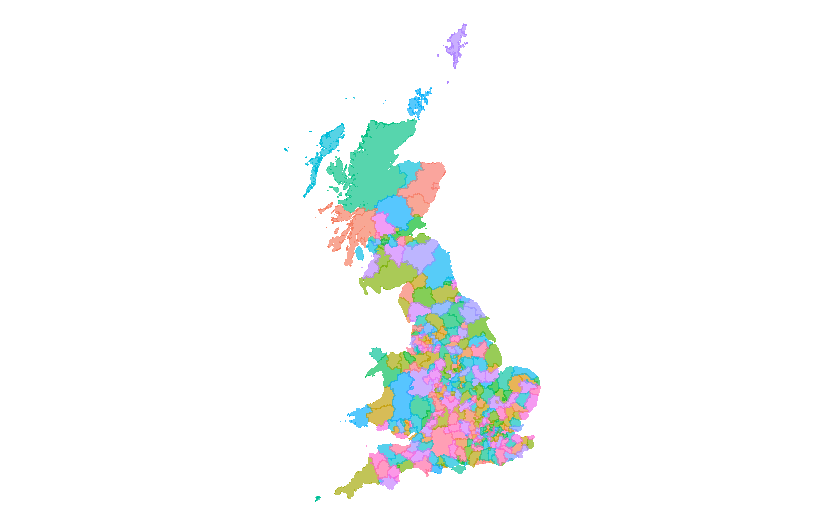
\includegraphics{./Maps_files/figure-pdf/map0a-1.pdf}

}

\end{figure}

Looking at the read-out above, each of the 380 regions have some
metadata associated, which are contained in each of the listed
attributes. It should be obvious that \texttt{objectid} is just a
sequence from 1 to 380. \texttt{lad15nm} turns out to be a list of names
of the regions -- I suspect \texttt{lad} for Local Authority District,
\texttt{15} for 2015 and \texttt{nm} for name -- and it is easy to
specify this as the name to use for the region when using \texttt{tidy}.

Now this can be plotted using \texttt{ggplot}, using \texttt{geometry}
for the \(x\) and \(y\) coordinates. The choice of fill colour is
determined by \texttt{fill} and we can set the colour of the lines by
\texttt{colour} (or \texttt{color}). The two extra arguments are for a
suitable blank style and to impose an appropriate ratio of height to
width.

Immediately, the awkward shape of the British Isles is apparent. (Note
this is a plot of Great Britain, and there is no Northern Ireland.) The
islands to the far north are somewhat unnecessary, although quite
rightly the inhabitants get a bit tired of being left off maps!
Nonetheless I'll do exactly the same by filtering out the polygons
associated with \texttt{Orkney\ Islands} and \texttt{Shetland\ Islands}.

Fewer Scottish Islands makes the graphs a lot clearer with little loss
of information, given the tiny number of transactions in the Orkneys and
the Shetlands, very far to the north.

In what follows we filter out the islands using

\begin{Shaded}
\begin{Highlighting}[]
\NormalTok{shape }\OtherTok{\textless{}{-}} \FunctionTok{read\_sf}\NormalTok{(}\AttributeTok{dsn=}\StringTok{"."}\NormalTok{, }\AttributeTok{layer=}\NormalTok{fle) }\SpecialCharTok{\%\textgreater{}\%}
  \FunctionTok{filter}\NormalTok{(}\SpecialCharTok{!}\NormalTok{lad15nm }\SpecialCharTok{\%in\%} \FunctionTok{c}\NormalTok{(}\StringTok{"Shetland Islands"}\NormalTok{,}\StringTok{"Orkney Islands"}\NormalTok{)) }\SpecialCharTok{\%\textgreater{}\%}
  \FunctionTok{mutate}\NormalTok{(}\AttributeTok{Country=}\FunctionTok{str\_sub}\NormalTok{(lad15cd, }\DecValTok{1}\NormalTok{, }\DecValTok{1}\NormalTok{), }\AttributeTok{.after=}\DecValTok{1}\NormalTok{)}
\end{Highlighting}
\end{Shaded}

where we also create an indicator of country using the first letter of
the code string.

So the country map is

\begin{Shaded}
\begin{Highlighting}[]
\NormalTok{shape }\SpecialCharTok{\%\textgreater{}\%}
  \FunctionTok{group\_by}\NormalTok{(Country) }\SpecialCharTok{\%\textgreater{}\%}
  \FunctionTok{summarise}\NormalTok{() }\SpecialCharTok{\%\textgreater{}\%}
  \FunctionTok{ggplot}\NormalTok{() }\SpecialCharTok{+}
  \FunctionTok{geom\_sf}\NormalTok{(}\FunctionTok{aes}\NormalTok{(}\AttributeTok{fill=}\NormalTok{Country), }\AttributeTok{color=}\StringTok{"grey77"}\NormalTok{, }\AttributeTok{linewidth=}\NormalTok{.}\DecValTok{25}\NormalTok{, }\AttributeTok{alpha=}\NormalTok{.}\DecValTok{66}\NormalTok{) }\SpecialCharTok{+}
  \FunctionTok{theme\_void}\NormalTok{()}
\end{Highlighting}
\end{Shaded}

\begin{figure}[H]

{\centering 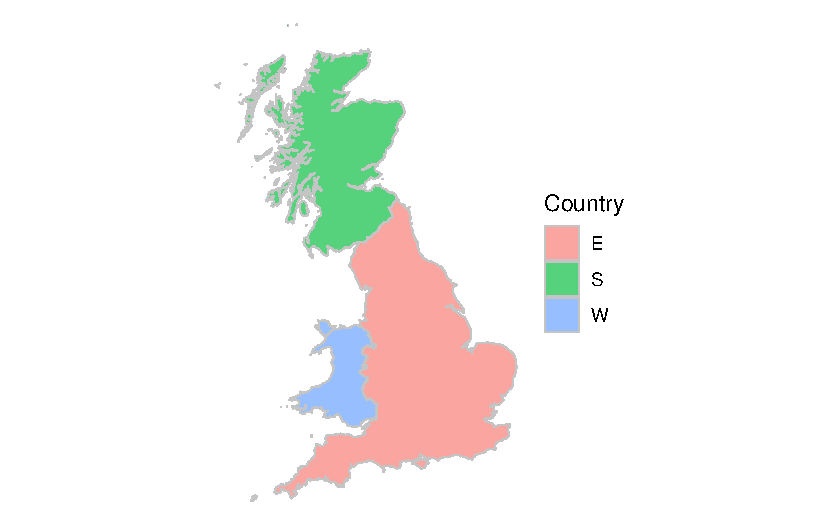
\includegraphics{./Maps_files/figure-pdf/map0d-1.pdf}

}

\end{figure}

Note the really nice feature -- if we group by something, in this case
country, we can summarise to amalgamate the geometries!

You may have noticed, one thing that that's missing on the LA graphs is
the boundaries. They aren't, they're just invisible. That's because I
set \texttt{colour\ =\ NA}, so I can fix that by choosing a colour and
making the lines very thin so they don't swamp the map, as in the
country one.

One further amendment, the \texttt{fill} is moved inside the
\texttt{aes()} specification and made conditional. \texttt{R} now
chooses unique colours for each of the regions.

Two things now need to be done to get the map colours right to
illustrate regional inflation rates. First we need to amalgamate some of
the Local Authority boundaries to the Land Registry definitions, and
second we need to assign the inflation rate to each area.

\hypertarget{inflation-data-and-regions}{%
\section{Inflation data and regions}\label{inflation-data-and-regions}}

We have a map, and we have that data in a form that is easy to
understand. If we can suitably attach an inflation rate to each area
then we can fill the individual areas with a colour unique to each
individual inflation rates.

Recall that the Land Registry areas aren't quite what we have, and will
need amalgamating. Bahaj, Foulis, and Pinter (2020) supplied me the
areas that needed amalgamating (and the inflation rates) using the
\href{https://en.wikipedia.org/wiki/ONS_coding_system}{ONS codes}. This
is contained in the metadata \texttt{lad15cd} above.

The data is structured in `wide' format with one row for each Land
Registry region. The details aren't very important for us now, but what
it means is I can manipulate it to get

\begin{Shaded}
\begin{Highlighting}[]
\CommentTok{\# Price data by Land Registry region, converted to long format}
\NormalTok{hp\_data }\OtherTok{\textless{}{-}} \FunctionTok{read\_excel}\NormalTok{(}\StringTok{"house\_price\_data\_figure\_1.xls"}\NormalTok{)  }\SpecialCharTok{\%\textgreater{}\%} 
  \FunctionTok{select}\NormalTok{(}\StringTok{"land\_reg\_region"}\NormalTok{, }\FunctionTok{starts\_with}\NormalTok{(}\StringTok{"e\_"}\NormalTok{), }\FunctionTok{starts\_with}\NormalTok{(}\StringTok{"av\_"}\NormalTok{)) }\SpecialCharTok{\%\textgreater{}\%} 
  \FunctionTok{pivot\_longer}\NormalTok{(}\AttributeTok{names\_to  =} \StringTok{"name"}\NormalTok{, }
               \AttributeTok{values\_to =} \StringTok{"lad15cd"}\NormalTok{, }
               \AttributeTok{cols      =} \FunctionTok{c}\NormalTok{(}\SpecialCharTok{{-}}\NormalTok{land\_reg\_region, }\SpecialCharTok{{-}}\FunctionTok{starts\_with}\NormalTok{(}\StringTok{"av\_"}\NormalTok{))) }\SpecialCharTok{\%\textgreater{}\%} 
  \FunctionTok{drop\_na}\NormalTok{() }\SpecialCharTok{\%\textgreater{}\%}
  \FunctionTok{select}\NormalTok{(land\_reg\_region, lad15cd, }\FunctionTok{starts\_with}\NormalTok{(}\StringTok{"av\_"}\NormalTok{)) }

\NormalTok{codes }\OtherTok{\textless{}{-}}\NormalTok{ hp\_data }\SpecialCharTok{\%\textgreater{}\%} 
  \FunctionTok{select}\NormalTok{(lad15cd, land\_reg\_region) }
\end{Highlighting}
\end{Shaded}

The important thing that the \texttt{pivot\_longer} achieves is that for
every \texttt{land\_reg\_region} I get a list of all the ONS codes that
makes up the Local Authority level. So if I look at
\texttt{buckinghamshire} as an example there are four ONS codes now
associated with it.

\begin{Shaded}
\begin{Highlighting}[]
\FunctionTok{filter}\NormalTok{(codes, land\_reg\_region }\SpecialCharTok{==} \StringTok{"buckinghamshire"}\NormalTok{)}
\end{Highlighting}
\end{Shaded}

\begin{verbatim}
# A tibble: 4 x 2
  lad15cd   land_reg_region
  <chr>     <chr>          
1 E07000004 buckinghamshire
2 E07000005 buckinghamshire
3 E07000006 buckinghamshire
4 E07000007 buckinghamshire
\end{verbatim}

Join these together

\begin{Shaded}
\begin{Highlighting}[]
\CommentTok{\# Join polygons defined by Land Registry regions}
\NormalTok{gg }\OtherTok{\textless{}{-}}\NormalTok{ shape }\SpecialCharTok{\%\textgreater{}\%}
  \FunctionTok{select}\NormalTok{(}\FunctionTok{starts\_with}\NormalTok{(}\FunctionTok{c}\NormalTok{(}\StringTok{"lad"}\NormalTok{,}\StringTok{"C"}\NormalTok{))) }\SpecialCharTok{\%\textgreater{}\%} 
  \FunctionTok{left\_join}\NormalTok{(codes, }\AttributeTok{by=}\StringTok{"lad15cd"}\NormalTok{) }\SpecialCharTok{\%\textgreater{}\%}
  \FunctionTok{group\_by}\NormalTok{(land\_reg\_region) }\SpecialCharTok{\%\textgreater{}\%}
  \FunctionTok{summarise}\NormalTok{() }
\end{Highlighting}
\end{Shaded}

which produces a match between the Land Registry and the Local Authority
areas, plus the inflation rates.

\hypertarget{inflation-in-grayscale}{%
\subsection{Inflation in grayscale}\label{inflation-in-grayscale}}

All the information required to plot the Land Registry-based regional
inflation rates is now available. As you can see from the
\texttt{buckinghamshire} data above, there are three average rates in
three different periods, so I'll focus on one, 2002-2007 to begin with.

First, augment the geographic data with the inflation data, and call
them something better.

\begin{Shaded}
\begin{Highlighting}[]
\NormalTok{gg }\SpecialCharTok{\%\textgreater{}\%}
  \FunctionTok{ggplot}\NormalTok{() }\SpecialCharTok{+}
  \FunctionTok{geom\_sf}\NormalTok{(}\FunctionTok{aes}\NormalTok{(}\AttributeTok{geometry=}\NormalTok{geometry, }\AttributeTok{fill=}\NormalTok{land\_reg\_region), }
          \AttributeTok{color=}\ConstantTok{NA}\NormalTok{, }\AttributeTok{alpha=}\NormalTok{.}\DecValTok{66}\NormalTok{, }\AttributeTok{show.legend =} \ConstantTok{FALSE}\NormalTok{) }\SpecialCharTok{+}
  \FunctionTok{theme\_void}\NormalTok{()}
\end{Highlighting}
\end{Shaded}

\begin{figure}[H]

{\centering 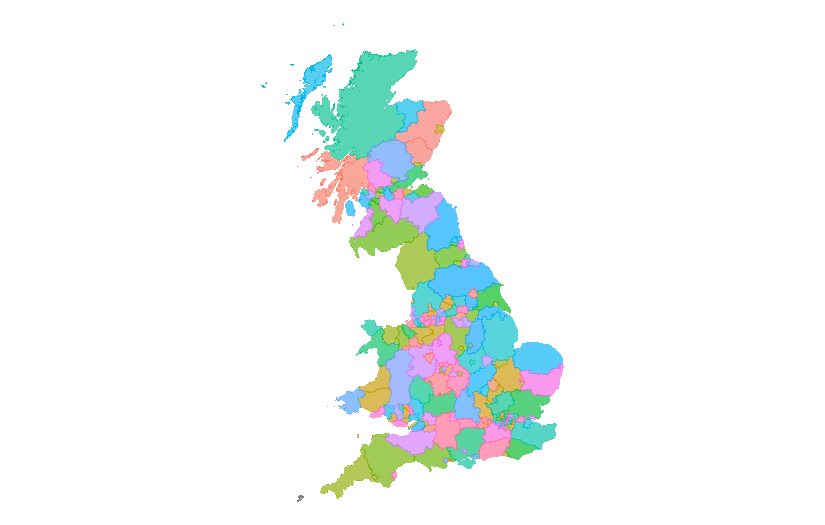
\includegraphics{./Maps_files/figure-pdf/unnamed-chunk-4-1.pdf}

}

\end{figure}

Then specify gray and put the legend at the bottom.

\begin{Shaded}
\begin{Highlighting}[]
\NormalTok{nms }\OtherTok{\textless{}{-}} \FunctionTok{gsub}\NormalTok{(}\StringTok{"av\_hp\_growth"}\NormalTok{, }\StringTok{"HPI"}\NormalTok{, }\FunctionTok{colnames}\NormalTok{(hp\_data))}

\NormalTok{hp\_data }\SpecialCharTok{\%\textgreater{}\%}
  \FunctionTok{rename\_all}\NormalTok{( }\SpecialCharTok{\textasciitilde{}}\NormalTok{ nms) }\SpecialCharTok{\%\textgreater{}\%}
  \FunctionTok{select}\NormalTok{(land\_reg\_region, }\FunctionTok{starts\_with}\NormalTok{(}\StringTok{"HPI"}\NormalTok{)) }\SpecialCharTok{\%\textgreater{}\%}
  \FunctionTok{distinct}\NormalTok{() }\SpecialCharTok{\%\textgreater{}\%}
  \FunctionTok{left\_join}\NormalTok{(gg) }\SpecialCharTok{\%\textgreater{}\%}
  \FunctionTok{ggplot}\NormalTok{() }\SpecialCharTok{+}
  \FunctionTok{geom\_sf}\NormalTok{(}\FunctionTok{aes}\NormalTok{(}\AttributeTok{geometry=}\NormalTok{geometry, }\AttributeTok{fill=}\NormalTok{HPI\_02\_07), }
          \AttributeTok{color=}\ConstantTok{NA}\NormalTok{, }\AttributeTok{alpha=}\NormalTok{.}\DecValTok{66}\NormalTok{, }\AttributeTok{show.legend =} \ConstantTok{TRUE}\NormalTok{) }\SpecialCharTok{+}
  \FunctionTok{theme\_void}\NormalTok{() }\SpecialCharTok{+}
  \FunctionTok{scale\_fill\_gradient}\NormalTok{(}\AttributeTok{low=}\FunctionTok{grey}\NormalTok{(}\FloatTok{0.9}\NormalTok{), }\AttributeTok{high=}\FunctionTok{grey}\NormalTok{(}\FloatTok{0.05}\NormalTok{)) }\SpecialCharTok{+}
  \FunctionTok{theme}\NormalTok{(}\AttributeTok{legend.direction =} \StringTok{"horizontal"}\NormalTok{, }
        \AttributeTok{legend.position  =} \FunctionTok{c}\NormalTok{(}\FloatTok{0.75}\NormalTok{,}\FloatTok{0.05}\NormalTok{),}
        \AttributeTok{legend.title     =} \FunctionTok{element\_blank}\NormalTok{())}
\end{Highlighting}
\end{Shaded}

\begin{verbatim}
Joining with `by = join_by(land_reg_region)`
\end{verbatim}

\begin{figure}[H]

{\centering 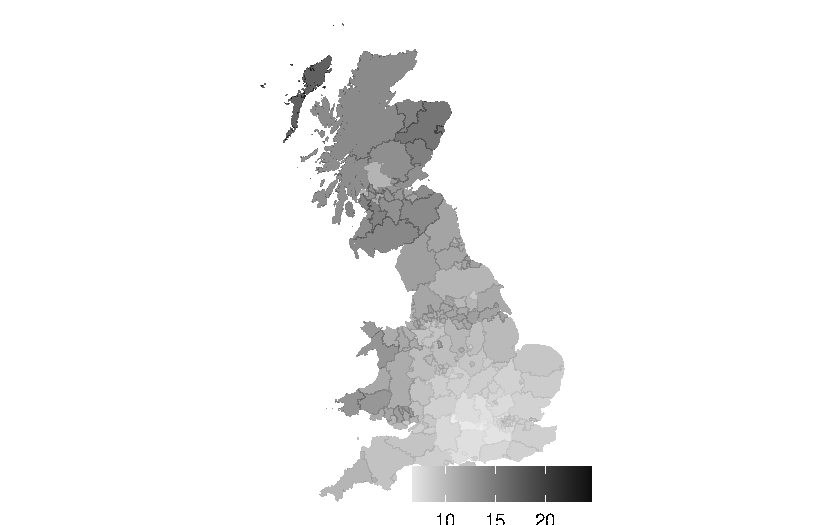
\includegraphics{./Maps_files/figure-pdf/unnamed-chunk-5-1.pdf}

}

\end{figure}

\part{Time}

\hypertarget{linear-rational-expectations-models}{%
\chapter{Linear rational expectations
models}\label{linear-rational-expectations-models}}

\hypertarget{introduction-2}{%
\section{Introduction}\label{introduction-2}}

How do we solve rational expectations models? Here I show how to
implement versions of the Blanchard and Kahn (1980) and Klein (2000)
solutions to linear rational expectations models in R. The
implementation is fairly general, and copes with singular models. It is
a very transparent implementation, with all the necessary code, and also
shows how to calculate and plot impulse responses.

\hypertarget{model}{%
\section{Model}\label{model}}

We take a simple New Keynesian model \[
\begin{align}
y_t    &= y_{t+1}^e-\frac{1}{\sigma} (i_t - \pi_{t+1}^e) + e_t^1 \\
\pi_t  &= \beta \pi_{t+1}^e + \kappa y_t + e_t^2 \\
i_t    &= \gamma i_{t-1} + (1-\gamma) \delta \pi_t + \varepsilon_t^3 \\ 
e_t^1  &= \rho_1 e_{t-1}^1 + \varepsilon_t^1 \\ 
e_t^2  &= \rho_2 e_{t-1}^2 + \varepsilon_t^2 
\end{align}
\] The model comprises a dynamic IS curve, a Phillips Curve and a policy
rule with smoothing. There are three shocks, two of which are
persistent. This we need to write in the general algebraic linear
state-space form: \[
E\begin{bmatrix} z_t \\ x_{t+1}^e \end{bmatrix} = A \begin{bmatrix} z_{t-1} \\ x_t \end{bmatrix} + B \varepsilon_t  
\] We map our variables to their algebraic equivalent as (\(z_t\),
\(x_t\)) \(=\) ((\(e^1_t\), \(e^2_t\), \(i_t\)), (\(y_t\), \(\pi_t\))).
Then the model in state-space form but including the matrix \(E\) is \[
\begin{bmatrix} 1 & 0 & 0 & 0 & 0 \\ 
                0 & 1 & 0 & 0 & 0 \\ 
                0 & 0 & 1 & 0 & 0 \\ 
                1 & 0 & -\frac{1}{\sigma} & 1 & \frac{1}{\sigma} \\ 
                0 & 1 & 0 & 0 & \beta
\end{bmatrix}
\begin{bmatrix} e^1_t \\ e^2_t \\ i_t \\ y^e_{t+1} \\ \pi^e_{t+1} \end{bmatrix} 
   = 
   \begin{bmatrix} \rho_1 & 0 & 0 & 0 & 0 \\ 
                0 & \rho_2 & 0 & 0 & 0 \\ 
                0 & 0 & \gamma & 0 & (1-\gamma)\delta \\ 
                0 & 0 & 0 & 1 & 0 \\ 
                0 & 0 & 0 & -\kappa & 1
   \end{bmatrix}
\begin{bmatrix} e^1_{t-1} \\ e^2_{t-1} \\ i_{t-1} \\ y_t \\ \pi_t \end{bmatrix}    
   + 
      \begin{bmatrix} 
                1 & 0 & 0  \\ 
                0 & 1 & 0 \\ 
                0 & 0 & 1 \\ 
                0 & 0 & 0 \\ 
                0 & 0 & 0 
   \end{bmatrix}
   \begin{bmatrix} \varepsilon^1_t \\ \varepsilon^2_t \\ \varepsilon^3_t \end{bmatrix}    
\] Anyone wanting to code up solutions should familiarize themselves
with this before continuing.

\hypertarget{coding-up-the-model-in-r}{%
\subsection{Coding up the model in R}\label{coding-up-the-model-in-r}}

Before we begin coding this in R, load the \texttt{tidyverse} libraries
so we can do impulse responses with our usual tool kit and then we can
forget about it.

\begin{Shaded}
\begin{Highlighting}[]
\FunctionTok{library}\NormalTok{(tidyverse)}
\end{Highlighting}
\end{Shaded}

Set the model parameters

\begin{Shaded}
\begin{Highlighting}[]
\NormalTok{nf    }\OtherTok{\textless{}{-}} \DecValTok{2}
\NormalTok{ns    }\OtherTok{\textless{}{-}} \DecValTok{5}
\NormalTok{ne    }\OtherTok{\textless{}{-}} \DecValTok{3}
\NormalTok{np    }\OtherTok{\textless{}{-}}\NormalTok{ ns}\SpecialCharTok{{-}}\NormalTok{nf}

\NormalTok{beta  }\OtherTok{\textless{}{-}} \FloatTok{0.99}   \CommentTok{\# Discount factor }
\NormalTok{sigma }\OtherTok{\textless{}{-}} \FloatTok{2.0}    \CommentTok{\# Elas. substitution}
\NormalTok{kappa }\OtherTok{\textless{}{-}} \FloatTok{0.075}  \CommentTok{\# Slope PC}
\NormalTok{delta }\OtherTok{\textless{}{-}} \FloatTok{1.5}    \CommentTok{\# Inflation feedback}
\NormalTok{gamma }\OtherTok{\textless{}{-}} \FloatTok{0.75}   \CommentTok{\# Smoothing}
\NormalTok{rho\_1 }\OtherTok{\textless{}{-}} \FloatTok{0.9}    \CommentTok{\# AR1}
\NormalTok{rho\_2 }\OtherTok{\textless{}{-}} \FloatTok{0.8}    \CommentTok{\# AR1}
\NormalTok{Omega }\OtherTok{\textless{}{-}} \FunctionTok{diag}\NormalTok{(}\FunctionTok{c}\NormalTok{(}\FloatTok{0.33}\NormalTok{,}\FloatTok{0.33}\NormalTok{,}\FloatTok{0.33}\NormalTok{)) }\CommentTok{\# SE of 3 shocks}
\end{Highlighting}
\end{Shaded}

Now define the model matrices `long hand' and some variable names, which
we put in \texttt{labels}.

\begin{Shaded}
\begin{Highlighting}[]
\NormalTok{labels }\OtherTok{\textless{}{-}} \FunctionTok{c}\NormalTok{(}\StringTok{"e\^{}1"}\NormalTok{,}\StringTok{"e\^{}2"}\NormalTok{,}\StringTok{"i"}\NormalTok{,}\StringTok{"y"}\NormalTok{,}\StringTok{"pi"}\NormalTok{)}

\NormalTok{E }\OtherTok{\textless{}{-}} \FunctionTok{matrix}\NormalTok{(}\DecValTok{0}\NormalTok{,ns,ns)}
\NormalTok{A }\OtherTok{\textless{}{-}} \FunctionTok{matrix}\NormalTok{(}\DecValTok{0}\NormalTok{,ns,ns)}
\NormalTok{B }\OtherTok{\textless{}{-}} \FunctionTok{diag}\NormalTok{(}\DecValTok{1}\NormalTok{,ns,ne)}

\CommentTok{\# Now put the equations in matrix form}
\FunctionTok{diag}\NormalTok{(E[}\DecValTok{1}\SpecialCharTok{:}\DecValTok{2}\NormalTok{,}\DecValTok{1}\SpecialCharTok{:}\DecValTok{2}\NormalTok{]) }\OtherTok{\textless{}{-}} \DecValTok{1}
\FunctionTok{diag}\NormalTok{(A[}\DecValTok{1}\SpecialCharTok{:}\DecValTok{2}\NormalTok{,}\DecValTok{1}\SpecialCharTok{:}\DecValTok{2}\NormalTok{]) }\OtherTok{\textless{}{-}} \FunctionTok{c}\NormalTok{(rho\_1, rho\_2)}

\NormalTok{E[}\DecValTok{3}\NormalTok{,}\DecValTok{3}\NormalTok{]             }\OtherTok{\textless{}{-}} \DecValTok{1} 
\NormalTok{E[}\DecValTok{4}\NormalTok{,}\FunctionTok{c}\NormalTok{(}\DecValTok{1}\NormalTok{, }\DecValTok{3}\NormalTok{, }\DecValTok{4}\NormalTok{, }\DecValTok{5}\NormalTok{)] }\OtherTok{\textless{}{-}} \FunctionTok{c}\NormalTok{(}\DecValTok{1}\NormalTok{, }\SpecialCharTok{{-}}\DecValTok{1}\SpecialCharTok{/}\NormalTok{sigma, }\DecValTok{1}\NormalTok{, }\DecValTok{1}\SpecialCharTok{/}\NormalTok{sigma)}
\NormalTok{E[}\DecValTok{5}\NormalTok{,}\FunctionTok{c}\NormalTok{(}\DecValTok{2}\NormalTok{, }\DecValTok{5}\NormalTok{)]       }\OtherTok{\textless{}{-}} \FunctionTok{c}\NormalTok{(}\DecValTok{1}\NormalTok{, beta)}

\NormalTok{A[}\DecValTok{3}\NormalTok{,}\FunctionTok{c}\NormalTok{(}\DecValTok{3}\NormalTok{, }\DecValTok{5}\NormalTok{)]       }\OtherTok{\textless{}{-}} \FunctionTok{c}\NormalTok{(gamma, (}\DecValTok{1}\SpecialCharTok{{-}}\NormalTok{gamma)}\SpecialCharTok{*}\NormalTok{delta)}
\NormalTok{A[}\DecValTok{4}\NormalTok{,}\DecValTok{4}\NormalTok{]             }\OtherTok{\textless{}{-}} \DecValTok{1}
\NormalTok{A[}\DecValTok{5}\NormalTok{,}\FunctionTok{c}\NormalTok{(}\DecValTok{4}\NormalTok{,}\DecValTok{5}\NormalTok{)]        }\OtherTok{\textless{}{-}} \FunctionTok{c}\NormalTok{(}\SpecialCharTok{{-}}\NormalTok{kappa, }\DecValTok{1}\NormalTok{)}
\end{Highlighting}
\end{Shaded}

where for example, \(E\) and \(A\) are \[  
E = \left[\begin{array}{r}1 &0 &0 &0 &0 \\0 &1 &0 &0 &0 \\0 &0 &1 &0 &0 \\1 &0 &-0.5 &1 &0.5 \\0 &1 &0 &0 &0.99 \\\end{array}\right] 
\] \[  
A = \left[\begin{array}{r}0.9 &0 &0 &0 &0 \\0 &0.8 &0 &0 &0 \\0 &0 &0.75 &0 &0.375 \\0 &0 &0 &1 &0 \\0 &0 &0 &-0.075 &1 \\\end{array}\right] 
\] Calculate the reduced form state-space model \[
\begin{bmatrix} z_t \\ x_{t+1}^e \end{bmatrix} = C \begin{bmatrix} z_{t-1} \\ x_t \end{bmatrix} + D \varepsilon_t  
\] which is done in R very simply as

\begin{Shaded}
\begin{Highlighting}[]
\NormalTok{C }\OtherTok{\textless{}{-}} \FunctionTok{solve}\NormalTok{(E,A)}
\NormalTok{D }\OtherTok{\textless{}{-}} \FunctionTok{solve}\NormalTok{(E,B)}
\end{Highlighting}
\end{Shaded}

Why can't we solve this for impulse responses?

The following function simulates the impulse responses of a model in a
loop within a loop\footnote{Sometimes a loop is the right way to do
  something.} and returns the time series in a suitably organised data
frame.

\begin{Shaded}
\begin{Highlighting}[]
\NormalTok{impulse\_responses }\OtherTok{\textless{}{-}} \ControlFlowTok{function}\NormalTok{(P, Q, Omega, labels, T) \{}
\NormalTok{  s   }\OtherTok{\textless{}{-}} \FunctionTok{matrix}\NormalTok{(}\DecValTok{0}\NormalTok{, }\FunctionTok{ncol}\NormalTok{(Q), }\DecValTok{1}\NormalTok{)}
\NormalTok{  z   }\OtherTok{\textless{}{-}} \FunctionTok{matrix}\NormalTok{(}\DecValTok{0}\NormalTok{, }\FunctionTok{nrow}\NormalTok{(Q), T)}
  \FunctionTok{rownames}\NormalTok{(z) }\OtherTok{\textless{}{-}}\NormalTok{ labels}
\NormalTok{  dza }\OtherTok{\textless{}{-}} \ConstantTok{NULL}
  \ControlFlowTok{for}\NormalTok{ (j }\ControlFlowTok{in} \DecValTok{1}\SpecialCharTok{:}\FunctionTok{ncol}\NormalTok{(Q)) \{}
\NormalTok{    s[j]  }\OtherTok{\textless{}{-}}\NormalTok{ Omega[j,j]}
\NormalTok{    z[,}\DecValTok{1}\NormalTok{] }\OtherTok{\textless{}{-}}\NormalTok{ Q }\SpecialCharTok{\%*\%}\NormalTok{ s}
    \ControlFlowTok{for}\NormalTok{ (i }\ControlFlowTok{in} \DecValTok{1}\SpecialCharTok{:}\NormalTok{(T}\DecValTok{{-}1}\NormalTok{)) \{}
\NormalTok{      z[,i}\SpecialCharTok{+}\DecValTok{1}\NormalTok{] }\OtherTok{\textless{}{-}}\NormalTok{ P }\SpecialCharTok{\%*\%}\NormalTok{ z[,i]}
\NormalTok{    \}}
\NormalTok{    s[j] }\OtherTok{\textless{}{-}} \DecValTok{0}
\NormalTok{    dz }\OtherTok{\textless{}{-}} \FunctionTok{as\_tibble}\NormalTok{(}\FunctionTok{t}\NormalTok{(z)) }\SpecialCharTok{\%\textgreater{}\%} 
      \FunctionTok{mutate}\NormalTok{(}\AttributeTok{Period =} \DecValTok{1}\SpecialCharTok{:}\NormalTok{T, }\AttributeTok{Shock =} \FunctionTok{paste0}\NormalTok{(}\StringTok{"epsilon\^{}"}\NormalTok{,j))}
\NormalTok{    dza }\OtherTok{\textless{}{-}} \FunctionTok{bind\_rows}\NormalTok{(dza,dz)}
\NormalTok{  \}}
  \FunctionTok{return}\NormalTok{(dza)}
\NormalTok{\}}
\end{Highlighting}
\end{Shaded}

A function to plot the impulses will be useful, so we create one.

\begin{Shaded}
\begin{Highlighting}[]
\NormalTok{response\_plot }\OtherTok{\textless{}{-}} \ControlFlowTok{function}\NormalTok{(series, title) \{}
  \FunctionTok{return}\NormalTok{(}\FunctionTok{pivot\_longer}\NormalTok{(series, }\AttributeTok{cols =} \SpecialCharTok{{-}}\FunctionTok{c}\NormalTok{(Period,Shock), }\AttributeTok{names\_to=}\StringTok{"Var"}\NormalTok{, }\AttributeTok{values\_to =} \StringTok{"Val"}\NormalTok{) }\SpecialCharTok{\%\textgreater{}\%}
           \FunctionTok{ggplot}\NormalTok{() }\SpecialCharTok{+}
           \FunctionTok{geom\_line}\NormalTok{(}\FunctionTok{aes}\NormalTok{(}\AttributeTok{x=}\NormalTok{Period, }\AttributeTok{y=}\NormalTok{Val, }\AttributeTok{group=}\NormalTok{Shock, }\AttributeTok{colour=}\NormalTok{Var), }\AttributeTok{show.legend=}\ConstantTok{FALSE}\NormalTok{) }\SpecialCharTok{+}
           \FunctionTok{facet\_grid}\NormalTok{(Shock}\SpecialCharTok{\textasciitilde{}}\NormalTok{Var, }\AttributeTok{scales=}\StringTok{"free"}\NormalTok{, }\AttributeTok{labeller=}\NormalTok{label\_parsed) }\SpecialCharTok{+}
           \FunctionTok{scale\_x\_continuous}\NormalTok{(}\AttributeTok{expand=}\FunctionTok{c}\NormalTok{(}\DecValTok{0}\NormalTok{,}\DecValTok{0}\NormalTok{)) }\SpecialCharTok{+}
           \FunctionTok{theme\_minimal}\NormalTok{() }\SpecialCharTok{+}
           \FunctionTok{labs}\NormalTok{(}\AttributeTok{title=}\NormalTok{title, }\AttributeTok{x=}\StringTok{""}\NormalTok{,}\AttributeTok{y=}\StringTok{""}\NormalTok{))}
\NormalTok{\}}
\end{Highlighting}
\end{Shaded}

Call the impulse response function using the model \(C\) and \(D\).

\begin{Shaded}
\begin{Highlighting}[]
\NormalTok{T }\OtherTok{\textless{}{-}} \DecValTok{25}
\NormalTok{z }\OtherTok{\textless{}{-}} \FunctionTok{impulse\_responses}\NormalTok{(C, D, Omega, labels, T)}
\end{Highlighting}
\end{Shaded}

and plot

\begin{Shaded}
\begin{Highlighting}[]
\FunctionTok{response\_plot}\NormalTok{(z, }\StringTok{"Impulse responses: Taylor rule"}\NormalTok{)}
\end{Highlighting}
\end{Shaded}

\begin{figure}[H]

{\centering 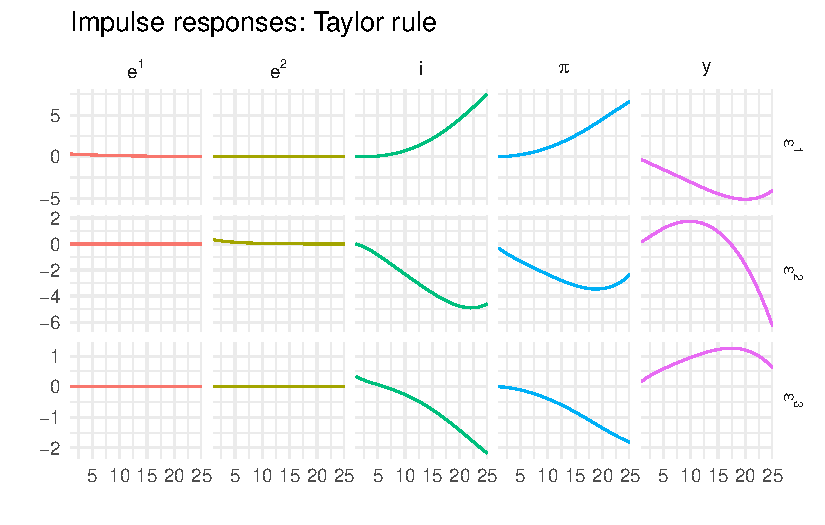
\includegraphics{./BK_files/figure-pdf/unnamed-chunk-4-1.pdf}

}

\end{figure}

Oh! That's not looking good. Let's try a few more periods.

\begin{Shaded}
\begin{Highlighting}[]
\NormalTok{T }\OtherTok{\textless{}{-}} \DecValTok{150}
\NormalTok{z }\OtherTok{\textless{}{-}} \FunctionTok{impulse\_responses}\NormalTok{(C, D, Omega, labels, T)}
\FunctionTok{response\_plot}\NormalTok{(z, }\StringTok{"Impulse responses: Taylor rule"}\NormalTok{)}
\end{Highlighting}
\end{Shaded}

\begin{figure}[H]

{\centering 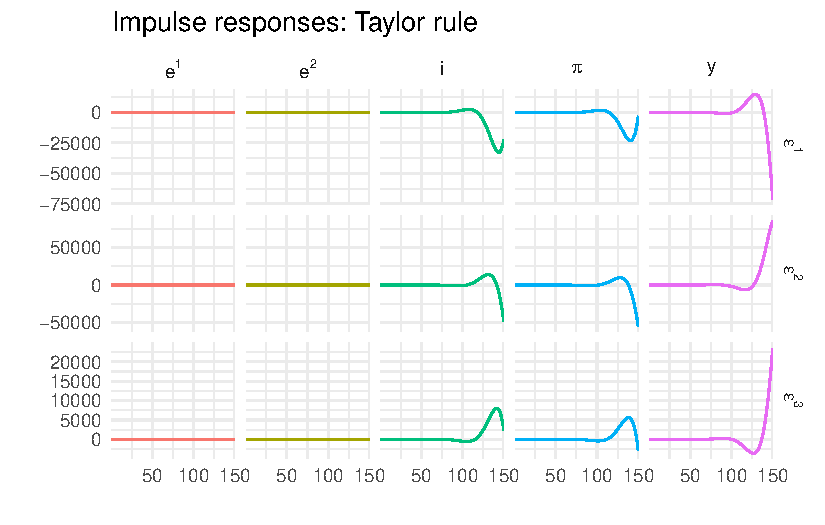
\includegraphics{./BK_files/figure-pdf/unnamed-chunk-5-1.pdf}

}

\end{figure}

This is clearly exploding. But it's rational -- we're solving forward so
expectations are always fulfilled. This is a key the insight of the
early rational expectations modellers -- rational isn't enough,
non-explosive is necessary too. Fortunately we know how to find this.

\hypertarget{bk80}{%
\section{Blanchard and Kahn (1980)}\label{bk80}}

To solve this model to give a unique \emph{stable} rational expectations
equilibrium, we appeal to the following. Consider the eigenvalue
decomposition \[
  MC=\Lambda M
\] where \(\Lambda\) is a diagonal matrix of \emph{eigenvalues} in
increasing absolute value and \(M\) is a non-singular matrix of
\emph{left eigenvectors}. Note that computer routines (including the one
in R) usually calculate \emph{right eigenvectors} such that
\(CV=V\Lambda\) and that \(M=V^{-1}\), so be aware of this in what
follows.

We can \emph{diagonalise} \(C\) and write it as \(C=M^{-1}\Lambda M\).
So pre-multiplying the reduced form model by \(M\) gives \[ 
M \begin{bmatrix} z_t \\ x_{t+1}^e \end{bmatrix} = \Lambda M \begin{bmatrix} z_{t-1} \\ x_t \end{bmatrix} + M D \varepsilon_t
\] Blanchard and Kahn (1980) (following Vaughan (1970)) show uniqueness
requires as many unstable eigenvalues as jump variables. To see this,
define \[
\begin{bmatrix} \xi_{t-1}^{s} \\  \xi_t^{u} \end{bmatrix}
  =  \begin{bmatrix} M_{11} & M_{12} \\  M_{21} & M_{22} \end{bmatrix}
      \begin{bmatrix} z_{t-1} \\  x_t \end{bmatrix}
\] Write the normalized model as \[
\begin{bmatrix} \xi_t^s \\ \xi_{t+1}^u \end{bmatrix}
 = \begin{bmatrix} \Lambda_s & 0 \\ 0 & \Lambda_u \end{bmatrix} 
\begin{bmatrix} \xi_{t-1}^s \\ \xi_t^u \end{bmatrix} +
\begin{bmatrix} M_1 \\ M_2 \end{bmatrix} D\varepsilon_t
\] where the eigenvalues are split into stable (\(\Lambda_s\)) and
unstable (\(\Lambda_u\)). If we ignore the stochastic bit for a moment
\[
\begin{bmatrix} \xi_t^s \\ \xi_{t+1}^u \end{bmatrix}
 = \begin{bmatrix} \Lambda_s & 0 \\ 0 & \Lambda_u \end{bmatrix} 
\begin{bmatrix} \xi_{t-1}^s \\ \xi_t^u \end{bmatrix}
\]

We seek a non-explosive solution, and this turns out to be easy to find
using the following

\begin{itemize}
\tightlist
\item
  The dynamics of \(\xi_t^u\) are determined by \(\Lambda_u\) and
  nothing else;
\item
  If they don't start at \(0\) they must explode;
\item
  This implies they must start at \(0\) and are always \(0\).
\end{itemize}

Thus the definition of the canonical variables necessarily implies \[
\begin{bmatrix} \xi_{t-1}^s \\  0 \end{bmatrix}
  =  \begin{bmatrix} M_{11} & M_{12} \\  M_{21} & M_{22} \end{bmatrix}
      \begin{bmatrix} z_{t-1} \\  x_t \end{bmatrix}
\]

From this it is clear that the jump variables themselves are only on the
saddle path if \[
   M_{21} z_{t-1} + M_{22} x_t = 0
\]

The rational solution implies that the jump variables are linearly
related to the predetermined ones through \[
\begin{aligned}
x_t &= -M_{22}^{-1} M_{21}z_{t-1} \\
    &= N z_{t-1}
\end{aligned}
\] We'll deal with the shocks in a moment.

\hypertarget{r-code}{%
\subsection{R code}\label{r-code}}

How do we do this in R? First, find the eigenvalue decomposition of
\(C\) using

\begin{Shaded}
\begin{Highlighting}[]
\NormalTok{m }\OtherTok{\textless{}{-}} \FunctionTok{eigen}\NormalTok{(C, }\AttributeTok{symmetric=}\ConstantTok{FALSE}\NormalTok{)}
\end{Highlighting}
\end{Shaded}

which yields

\begin{verbatim}
eigen() decomposition
$values
[1] 1.0715518+0.092734i 1.0715518-0.092734i 0.9000000+0.000000i
[4] 0.8000000+0.000000i 0.6548762+0.000000i

$vectors
                      [,1]                  [,2]         [,3]           [,4]
[1,]  0.0000000+0.0000000i  0.0000000+0.0000000i 0.2854942+0i  0.00000000+0i
[2,]  0.0000000+0.0000000i  0.0000000+0.0000000i 0.0000000+0i  0.09783896+0i
[3,]  0.1599159-0.5089425i  0.1599159+0.5089425i 0.7830500+0i  0.49622464+0i
[4,] -0.6991064+0.0000000i -0.6991064+0.0000000i 0.4552131+0i -0.86012270+0i
[5,]  0.2629802-0.3968579i  0.2629802+0.3968579i 0.3132200+0i  0.06616328+0i
              [,5]
[1,]  0.0000000+0i
[2,]  0.0000000+0i
[3,]  0.6351203+0i
[4,] -0.7554249+0i
[5,] -0.1611069+0i
\end{verbatim}

However this calculates \emph{right} eigenvectors. We will need to
invert it for left ones. Given the number of jump variables in the model
satisfies the Blanchard-Kahn conditions of as many unstable roots
(1.072+0.093i, 1.072-0.093i) as jump variables (2) we can calculate the
reaction function from the eigenvectors

\begin{Shaded}
\begin{Highlighting}[]
\NormalTok{iz }\OtherTok{\textless{}{-}} \DecValTok{1}\SpecialCharTok{:}\NormalTok{np}
\NormalTok{ix }\OtherTok{\textless{}{-}}\NormalTok{ (np}\SpecialCharTok{+}\DecValTok{1}\NormalTok{)}\SpecialCharTok{:}\NormalTok{ns}
\NormalTok{M  }\OtherTok{\textless{}{-}} \FunctionTok{solve}\NormalTok{(m}\SpecialCharTok{$}\NormalTok{vectors[,ns}\SpecialCharTok{:}\DecValTok{1}\NormalTok{])        }\CommentTok{\# Invert \& reverse order for increasing abs value}
\NormalTok{N  }\OtherTok{\textless{}{-}} \SpecialCharTok{{-}}\FunctionTok{Re}\NormalTok{(}\FunctionTok{solve}\NormalTok{(M[ix,ix], M[ix,iz])) }\CommentTok{\# Drop tiny complex bits (if any)}
\end{Highlighting}
\end{Shaded}

where \texttt{iz} are the indices of the first \texttt{np} variables and
\texttt{ix} those of the remaining \texttt{nf} ones.

\hypertarget{stochastic-part}{%
\subsection{Stochastic part}\label{stochastic-part}}

What about the shocks? Assume the stochastic reaction function is \[
  x_t = N z_{t-1} + G \varepsilon_t 
\] Following Andrew P. Blake (2004), note that \(x_{t+1}^e = N z_t\) as
the expected value of \(\varepsilon_{t+1}=0\), meaning we can write \[
 Nz_t = C_{21}z_{t-1} + C_{22} x_t + D_2 \varepsilon_t
\] or \[
 N\left( C_{11}z_{t-1} + C_{12}x_t + D_1 \varepsilon_t\right) = C_{21}z_{t-1} + C_{22} x_t + D_2 \varepsilon_t
\] Gathering terms we obtain \[
  (C_{22} - N C_{12}) x_t = (NC_{11} - C_{21}) z_{t-1} + (N D_1 - D_2) \varepsilon_t
\] which implies \[
G=(C_{22} - N C_{12})^{-1}(N D_1 - D_2) 
\] Notice it also implies
\(N = (C_{22} - N C_{12})^{-1}(NC_{11} - C_{21})\). It is this fixed
point nature of the solution for \(N\) -- which in turn implies the
quadratic matrix equation \(C_{21} = NC_{11} - C_{22}N + N C_{12}N\) --
that means we need to use the Blanchard and Kahn (1980) method in the
first place.

\hypertarget{r-code-1}{%
\subsection{R code}\label{r-code-1}}

All of this means that

\begin{Shaded}
\begin{Highlighting}[]
\NormalTok{G }\OtherTok{\textless{}{-}} \FunctionTok{solve}\NormalTok{((C[ix,ix] }\SpecialCharTok{{-}}\NormalTok{ N }\SpecialCharTok{\%*\%}\NormalTok{ C[iz,ix]), (N }\SpecialCharTok{\%*\%}\NormalTok{ D[iz,]}\SpecialCharTok{{-}}\NormalTok{ D[ix,]))}
\end{Highlighting}
\end{Shaded}

so for our model and parameters \(N\) and \(G\) are

\begin{Shaded}
\begin{Highlighting}[]
\NormalTok{N}
\end{Highlighting}
\end{Shaded}

\begin{verbatim}
        [,1]      [,2]       [,3]
[1,] 4.85680 -2.758647 -1.1894200
[2,] 1.79286  1.962790 -0.2536635
\end{verbatim}

\begin{Shaded}
\begin{Highlighting}[]
\NormalTok{G}
\end{Highlighting}
\end{Shaded}

\begin{verbatim}
         [,1]      [,2]      [,3]
[1,] 5.396445 -3.448309 -1.585893
[2,] 1.992067  2.453488 -0.338218
\end{verbatim}

The `fixed point' check is that the following should be the same as
\(N\)

\begin{Shaded}
\begin{Highlighting}[]
\FunctionTok{solve}\NormalTok{((C[ix,ix] }\SpecialCharTok{{-}}\NormalTok{ N }\SpecialCharTok{\%*\%}\NormalTok{ C[iz,ix]), (N }\SpecialCharTok{\%*\%}\NormalTok{ C[iz,iz]}\SpecialCharTok{{-}}\NormalTok{ C[ix,iz]))}
\end{Highlighting}
\end{Shaded}

\begin{verbatim}
        [,1]      [,2]       [,3]
[1,] 4.85680 -2.758647 -1.1894200
[2,] 1.79286  1.962790 -0.2536635
\end{verbatim}

which it is.

The solved model is finally \[
\begin{align}
\begin{bmatrix} z_t \\ x_t \end{bmatrix} &= \begin{bmatrix} C_{11}+C_{12}N & 0 \\ N & 0 \end{bmatrix} \begin{bmatrix} z_{t-1} \\ x_{t-1} \end{bmatrix} + \begin{bmatrix} D_1+C_{12}G \\ G \end{bmatrix} \varepsilon_t \\
 &= P \begin{bmatrix} z_{t-1} \\ x_{t-1} \end{bmatrix} + Q \varepsilon_t
\end{align}
\] which can be coded as

\begin{Shaded}
\begin{Highlighting}[]
\NormalTok{P  }\OtherTok{\textless{}{-}} \FunctionTok{cbind}\NormalTok{(}\FunctionTok{rbind}\NormalTok{((C[iz,iz] }\SpecialCharTok{+}\NormalTok{ C[iz,ix] }\SpecialCharTok{\%*\%}\NormalTok{ N), N), }\FunctionTok{matrix}\NormalTok{(}\DecValTok{0}\NormalTok{,ns,nf))}
\NormalTok{Q  }\OtherTok{\textless{}{-}} \FunctionTok{rbind}\NormalTok{(D[iz,] }\SpecialCharTok{+}\NormalTok{ C[iz,ix] }\SpecialCharTok{\%*\%}\NormalTok{ G, G)}
\end{Highlighting}
\end{Shaded}

\hypertarget{digression-right-eigenvector-version}{%
\subsection{Digression -- right eigenvector
version}\label{digression-right-eigenvector-version}}

It turns out that we could use the output from the standard
eigenvalue/vector routine directly by exploiting the following. This
time, let \(M\) be the matrix of \emph{right eigenvectors} so \[
  C M = M \Lambda \text{  or  } C = M\Lambda M^{-1}
\]\\
and \[
\begin{bmatrix} M_{11} & M_{12} \\ M_{21} & M_{22} \end{bmatrix}
\begin{bmatrix} \xi_{t-1}^s \\ \xi_t^u \end{bmatrix}
 = 
\begin{bmatrix} z_{t-1} \\ x_t \end{bmatrix}
\]

Written this way around, if \(\xi_t^{u}=0\) \(\forall\ t\) then (again
ignoring stochastics)

\[
  M_{11} \xi_{t-1}^s = z_{t-1}, \ M_{21}\xi_t^s = x_t 
\]

\[
   \Rightarrow x_t = M_{21} M_{11}^{-1} z_t
\] so

\begin{Shaded}
\begin{Highlighting}[]
\NormalTok{M }\OtherTok{\textless{}{-}}\NormalTok{ m}\SpecialCharTok{$}\NormalTok{vectors[,ns}\SpecialCharTok{:}\DecValTok{1}\NormalTok{]            }\CommentTok{\# Don\textquotesingle{}t invert as already right vectors, but reorder}
\FunctionTok{Re}\NormalTok{(M[ix,iz] }\SpecialCharTok{\%*\%} \FunctionTok{solve}\NormalTok{(M[iz,iz])) }\CommentTok{\# Again, drop tiny complex bits}
\end{Highlighting}
\end{Shaded}

\begin{verbatim}
        [,1]      [,2]       [,3]
[1,] 4.85680 -2.758647 -1.1894200
[2,] 1.79286  1.962790 -0.2536635
\end{verbatim}

The result is identical. This method is particularly useful if there are
fewer predetermined variables than jumps as the matrix we need to invert
is of the same dimension as the predetermined variables this way round.

\hypertarget{impulse-responses}{%
\subsection{Impulse responses}\label{impulse-responses}}

We now call the impulse response function using the model solved for
rational expectations.

\begin{Shaded}
\begin{Highlighting}[]
\NormalTok{T }\OtherTok{\textless{}{-}} \DecValTok{25}
\NormalTok{z }\OtherTok{\textless{}{-}} \FunctionTok{impulse\_responses}\NormalTok{(P, Q, Omega, labels, T)}
\end{Highlighting}
\end{Shaded}

Now plot these responses

\begin{Shaded}
\begin{Highlighting}[]
\FunctionTok{response\_plot}\NormalTok{(z, }\StringTok{"Impulse responses: Taylor rule"}\NormalTok{)}
\end{Highlighting}
\end{Shaded}

\begin{figure}[H]

{\centering 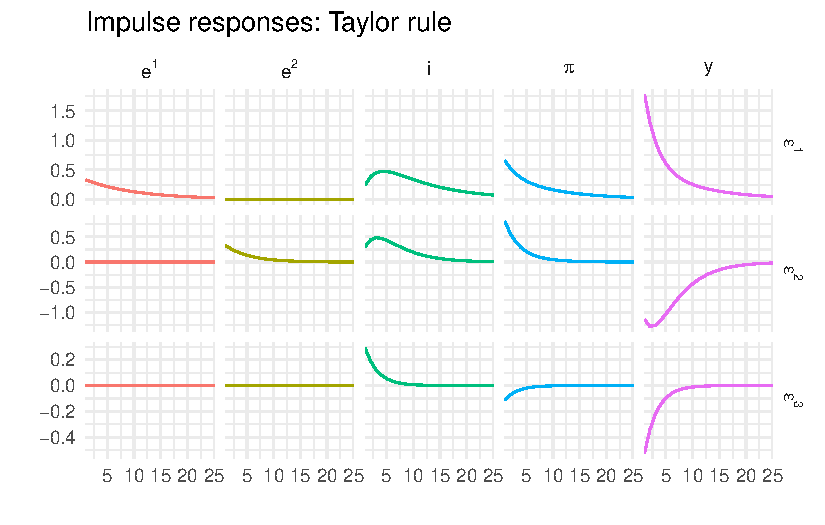
\includegraphics{./BK_files/figure-pdf/unnamed-chunk-13-1.pdf}

}

\end{figure}

Now, that looks better! It is no longer explosive. It also makes
complete economic sense, which you can verify by going through the
dynamics of the different demand, supply and monetary shocks.

\hypertarget{generalized-solution}{%
\section{Generalized solution}\label{generalized-solution}}

Sometimes for a model \(E\) is singular. A more general solution was
proposed by Klein (2000), that doesn't require \(E\) to be non-singular.
This uses a generalized Schur decomposition instead of an eigenvalue one
and is applied to the structural model represented by the matrix pencil
\((A,E)\), and is considered much more numerically stable (see Pappas,
Laub, and Sandell (1980)). The generalized Schur form of \((A,E)\) is
\((QTZ', QSZ')\), so we can write the model as \[
E \begin{bmatrix} z_t \\ x_{t+1}^e \end{bmatrix} \equiv QTZ' \begin{bmatrix} z_t \\ x_{t+1}^e \end{bmatrix} \equiv QT \begin{bmatrix} \xi_t^s \\ \xi_{t+1}^u \end{bmatrix} 
\] and \[
A \begin{bmatrix} z_{t-1} \\ x_t \end{bmatrix} \equiv QSZ' \begin{bmatrix} z_{t-1} \\ x_t \end{bmatrix} \equiv QS\begin{bmatrix} \xi_{t-1}^s \\ \xi_t^u \end{bmatrix} 
\] so the model pre-multiplied by \(Q'\) is \[
T \begin{bmatrix} \xi_{t+1}^s \\ \xi_{t+1}^u \end{bmatrix} = S \begin{bmatrix} \xi_t^s \\ \xi_t^u \end{bmatrix} + Q'B\varepsilon_t
\]

We use the function \texttt{gqz} from the library \texttt{geigen} for
this

\begin{Shaded}
\begin{Highlighting}[]
\NormalTok{d }\OtherTok{\textless{}{-}}\NormalTok{ geigen}\SpecialCharTok{::}\FunctionTok{gqz}\NormalTok{(A, E, }\AttributeTok{sort=}\StringTok{"S"}\NormalTok{) }\CommentTok{\# Option "S" puts the stable roots first}
\end{Highlighting}
\end{Shaded}

We can check that this is actually saddle path using \texttt{gevalues()}
to get all the eigenvalues from the generalized Schur decomposition, and
the unstable ones are

\begin{Shaded}
\begin{Highlighting}[]
\NormalTok{e }\OtherTok{\textless{}{-}}\NormalTok{ geigen}\SpecialCharTok{::}\FunctionTok{gevalues}\NormalTok{(d)}
\NormalTok{e[}\FunctionTok{abs}\NormalTok{(e) }\SpecialCharTok{\textgreater{}} \DecValTok{1}\NormalTok{]}
\end{Highlighting}
\end{Shaded}

\begin{verbatim}
[1] 1.071552+0.092734i 1.071552-0.092734i
\end{verbatim}

The number of \emph{stable} roots is returned in \texttt{d\$sdim} which
is 3.

We then modify our solution function to calculate \texttt{Ns} and
\texttt{Gs} using the matrix \texttt{Z} and a generalized version of the
formula for \(G\) and calculate the reduced form model \texttt{Ps} and
`Q which are \[
\begin{align}
    N_s &= Z_{21} Z_{11}^{-1} \\
    H   &= (E_{11} + E_{12} N_s)^{-1} \\
    W   &= (E_{21} + E_{22} N_s) H\\
    G_s &= (A_{22} - W A_{12})^{-1} (W B_1 - B_2) \\
    P_s &= H (A_{11} + A_{12} N_s) \\
    Q_s &= H (B_1 + A_{12} G_s)
\end{align}
\] Verify this yourself with a bit of matrix algebra!

The R code for this is

\begin{Shaded}
\begin{Highlighting}[]
\NormalTok{solveGenBK }\OtherTok{\textless{}{-}} \ControlFlowTok{function}\NormalTok{(E,A,B,n) \{}
\NormalTok{  d  }\OtherTok{\textless{}{-}}\NormalTok{ geigen}\SpecialCharTok{::}\FunctionTok{gqz}\NormalTok{(A, E, }\AttributeTok{sort=}\StringTok{"S"}\NormalTok{) }
\NormalTok{  np }\OtherTok{\textless{}{-}}\NormalTok{ d}\SpecialCharTok{$}\NormalTok{sdim}
\NormalTok{  ns }\OtherTok{\textless{}{-}} \FunctionTok{nrow}\NormalTok{(E)}
  \FunctionTok{print}\NormalTok{(}\FunctionTok{paste}\NormalTok{(}\StringTok{"Number of unstable roots is"}\NormalTok{, ns}\SpecialCharTok{{-}}\NormalTok{np))}
  \ControlFlowTok{if}\NormalTok{ (n }\SpecialCharTok{==}\NormalTok{ np) \{}
\NormalTok{    iz }\OtherTok{\textless{}{-}} \DecValTok{1}\SpecialCharTok{:}\NormalTok{n}
\NormalTok{    ix }\OtherTok{\textless{}{-}}\NormalTok{ (n}\SpecialCharTok{+}\DecValTok{1}\NormalTok{)}\SpecialCharTok{:}\NormalTok{ns}
\NormalTok{    Ns }\OtherTok{\textless{}{-}}\NormalTok{ d}\SpecialCharTok{$}\NormalTok{Z[ix,iz] }\SpecialCharTok{\%*\%} \FunctionTok{solve}\NormalTok{(d}\SpecialCharTok{$}\NormalTok{Z[iz,iz])}
\NormalTok{    H  }\OtherTok{\textless{}{-}} \FunctionTok{solve}\NormalTok{(E[iz,iz] }\SpecialCharTok{+}\NormalTok{ E[iz,ix] }\SpecialCharTok{\%*\%}\NormalTok{ Ns)}
\NormalTok{    W  }\OtherTok{\textless{}{-}}\NormalTok{ (E[ix,iz] }\SpecialCharTok{+}\NormalTok{ E[ix,ix] }\SpecialCharTok{\%*\%}\NormalTok{ Ns) }\SpecialCharTok{\%*\%}\NormalTok{ H}
\NormalTok{    Gs }\OtherTok{\textless{}{-}} \FunctionTok{solve}\NormalTok{((A[ix,ix] }\SpecialCharTok{{-}}\NormalTok{ W }\SpecialCharTok{\%*\%}\NormalTok{ A[iz,ix]), (W }\SpecialCharTok{\%*\%}\NormalTok{ B[iz,] }\SpecialCharTok{{-}}\NormalTok{ B[ix,]))}
\NormalTok{    As }\OtherTok{\textless{}{-}}\NormalTok{ H }\SpecialCharTok{\%*\%}\NormalTok{ (A[iz,iz] }\SpecialCharTok{+}\NormalTok{ A[iz,ix] }\SpecialCharTok{\%*\%}\NormalTok{ Ns)}
\NormalTok{    Bs }\OtherTok{\textless{}{-}}\NormalTok{ H }\SpecialCharTok{\%*\%}\NormalTok{ (B[iz,] }\SpecialCharTok{+}\NormalTok{ A[iz,ix] }\SpecialCharTok{\%*\%}\NormalTok{ Gs)}
    \FunctionTok{return}\NormalTok{(}\FunctionTok{list}\NormalTok{(}\AttributeTok{P=}\FunctionTok{cbind}\NormalTok{(}\FunctionTok{rbind}\NormalTok{(As,Ns),}\FunctionTok{matrix}\NormalTok{(}\DecValTok{0}\NormalTok{,ns,ns}\SpecialCharTok{{-}}\NormalTok{n)), }\AttributeTok{Q=}\FunctionTok{rbind}\NormalTok{(Bs, Gs)))}
\NormalTok{    \} }
  \ControlFlowTok{else}\NormalTok{ \{ }
    \FunctionTok{return}\NormalTok{(}\SpecialCharTok{{-}}\DecValTok{1}\NormalTok{) }
\NormalTok{    \}}
\NormalTok{\}}
\end{Highlighting}
\end{Shaded}

Using this on our original model gives

\begin{Shaded}
\begin{Highlighting}[]
\NormalTok{S  }\OtherTok{\textless{}{-}} \FunctionTok{solveGenBK}\NormalTok{(E,A,B,np)}
\end{Highlighting}
\end{Shaded}

\begin{verbatim}
[1] "Number of unstable roots is 2"
\end{verbatim}

\begin{Shaded}
\begin{Highlighting}[]
\NormalTok{Ps }\OtherTok{\textless{}{-}}\NormalTok{ S}\SpecialCharTok{$}\NormalTok{P}
\NormalTok{Qs }\OtherTok{\textless{}{-}}\NormalTok{ S}\SpecialCharTok{$}\NormalTok{Q}
\end{Highlighting}
\end{Shaded}

and comparing \texttt{Ps} and \texttt{Qs} with \texttt{P} and \texttt{Q}
obtained using Blanchard-Kahn we find

\begin{Shaded}
\begin{Highlighting}[]
\FunctionTok{round}\NormalTok{(}\FunctionTok{max}\NormalTok{(}\FunctionTok{abs}\NormalTok{(P}\SpecialCharTok{{-}}\NormalTok{Ps), }\FunctionTok{abs}\NormalTok{(Q}\SpecialCharTok{{-}}\NormalTok{Qs)), }\DecValTok{12}\NormalTok{)}
\end{Highlighting}
\end{Shaded}

\begin{verbatim}
[1] 0
\end{verbatim}

They are, as expected, the same -- at least up to 12 decimal places,
which should be enough.

\hypertarget{singular-models-optimal-policy}{%
\section{Singular models: optimal
policy}\label{singular-models-optimal-policy}}

However, this is an easy test. What we need is to use a model that can't
be solved using the BK method. Under optimal policy, the interest rate
instrument rule is replaced with a targeting rule, so that \[
  \pi_t = -\mu \Delta y_t - \varepsilon^3_t
\] for some value of \(\mu\) that reflects the optimal trade-off between
output (gap) growth and inflation, and we've included a disturbance
which we can loosely describe as a monetary policy shock. We modify the
model above by dropping the Taylor rule in favour of the targeting rule.
This requires a lagged value of \(y\) to be created. The following does
the trick

\begin{Shaded}
\begin{Highlighting}[]
\NormalTok{nf }\OtherTok{\textless{}{-}} \DecValTok{2}
\NormalTok{ne }\OtherTok{\textless{}{-}} \DecValTok{3}
\NormalTok{ns }\OtherTok{\textless{}{-}} \DecValTok{6}      \CommentTok{\# One extra state}
\NormalTok{np }\OtherTok{\textless{}{-}}\NormalTok{ ns}\SpecialCharTok{{-}}\NormalTok{nf}
\NormalTok{mu }\OtherTok{\textless{}{-}} \FloatTok{0.75}   \CommentTok{\# Representative trade{-}off}

\NormalTok{labels }\OtherTok{\textless{}{-}} \FunctionTok{c}\NormalTok{(}\StringTok{"e\^{}1"}\NormalTok{,}\StringTok{"e\^{}2"}\NormalTok{,}\StringTok{"ylag"}\NormalTok{,}\StringTok{"i"}\NormalTok{,}\StringTok{"y"}\NormalTok{,}\StringTok{"pi"}\NormalTok{) }\CommentTok{\# New variable order}

\NormalTok{E }\OtherTok{\textless{}{-}} \FunctionTok{matrix}\NormalTok{(}\DecValTok{0}\NormalTok{,ns,ns)}
\NormalTok{A }\OtherTok{\textless{}{-}}\NormalTok{ E}
\NormalTok{B }\OtherTok{\textless{}{-}} \FunctionTok{matrix}\NormalTok{(}\DecValTok{0}\NormalTok{,ns,ne)}
\NormalTok{B[}\DecValTok{1}\NormalTok{,}\DecValTok{1}\NormalTok{] }\OtherTok{\textless{}{-}} \DecValTok{1}
\NormalTok{B[}\DecValTok{2}\NormalTok{,}\DecValTok{2}\NormalTok{] }\OtherTok{\textless{}{-}} \DecValTok{1}
\NormalTok{B[}\DecValTok{4}\NormalTok{,}\DecValTok{3}\NormalTok{] }\OtherTok{\textless{}{-}} \SpecialCharTok{{-}}\DecValTok{1}

\FunctionTok{diag}\NormalTok{(E[}\DecValTok{1}\SpecialCharTok{:}\DecValTok{3}\NormalTok{,}\DecValTok{1}\SpecialCharTok{:}\DecValTok{3}\NormalTok{]) }\OtherTok{\textless{}{-}} \DecValTok{1}
\FunctionTok{diag}\NormalTok{(A[}\DecValTok{1}\SpecialCharTok{:}\DecValTok{2}\NormalTok{,}\DecValTok{1}\SpecialCharTok{:}\DecValTok{2}\NormalTok{]) }\OtherTok{\textless{}{-}} \FunctionTok{c}\NormalTok{(rho\_1, rho\_2)}
\NormalTok{A[}\DecValTok{3}\NormalTok{,}\DecValTok{5}\NormalTok{]           }\OtherTok{\textless{}{-}} \DecValTok{1}

\NormalTok{E[}\DecValTok{4}\NormalTok{,}\DecValTok{3}\NormalTok{]           }\OtherTok{\textless{}{-}} \DecValTok{1}
\NormalTok{A[}\DecValTok{4}\NormalTok{,}\FunctionTok{c}\NormalTok{(}\DecValTok{3}\NormalTok{, }\DecValTok{6}\NormalTok{)]     }\OtherTok{\textless{}{-}} \FunctionTok{c}\NormalTok{(}\DecValTok{1}\NormalTok{, }\SpecialCharTok{{-}}\DecValTok{1}\SpecialCharTok{/}\NormalTok{mu)}

\NormalTok{E[}\DecValTok{5}\NormalTok{,}\FunctionTok{c}\NormalTok{(}\DecValTok{1}\NormalTok{, }\DecValTok{4}\NormalTok{, }\DecValTok{5}\NormalTok{, }\DecValTok{6}\NormalTok{)] }\OtherTok{\textless{}{-}} \FunctionTok{c}\NormalTok{(}\DecValTok{1}\NormalTok{, }\SpecialCharTok{{-}}\DecValTok{1}\SpecialCharTok{/}\NormalTok{sigma, }\DecValTok{1}\NormalTok{, }\DecValTok{1}\SpecialCharTok{/}\NormalTok{sigma)}
\NormalTok{A[}\DecValTok{5}\NormalTok{,}\DecValTok{5}\NormalTok{]           }\OtherTok{\textless{}{-}} \DecValTok{1}

\NormalTok{E[}\DecValTok{6}\NormalTok{,}\FunctionTok{c}\NormalTok{(}\DecValTok{2}\NormalTok{, }\DecValTok{6}\NormalTok{)]     }\OtherTok{\textless{}{-}} \FunctionTok{c}\NormalTok{(}\DecValTok{1}\NormalTok{, beta)}
\NormalTok{A[}\DecValTok{6}\NormalTok{,}\FunctionTok{c}\NormalTok{(}\DecValTok{5}\NormalTok{, }\DecValTok{6}\NormalTok{)]     }\OtherTok{\textless{}{-}} \FunctionTok{c}\NormalTok{(}\SpecialCharTok{{-}}\NormalTok{kappa, }\DecValTok{1}\NormalTok{)}
\end{Highlighting}
\end{Shaded}

The new \(E\) and \(A\) system matrices are then \[  
E = \left[\begin{array}{r}1 &0 &0 &0 &0 &0 \\0 &1 &0 &0 &0 &0 \\0 &0 &1 &0 &0 &0 \\0 &0 &1 &0 &0 &0 \\1 &0 &0 &-0.5 &1 &0.5 \\0 &1 &0 &0 &0 &0.99 \\\end{array}\right] 
\] \[  
A = \left[\begin{array}{r}0.9 &0 &0 &0 &0 &0 \\0 &0.8 &0 &0 &0 &0 \\0 &0 &0 &0 &1 &0 \\0 &0 &1 &0 &0 &-1.333 \\0 &0 &0 &0 &1 &0 \\0 &0 &0 &0 &-0.075 &1 \\\end{array}\right] 
\] Now we have a singular model. The matrix \(E\) is clearly singular as
rows 3 and 4 are identical. But we have a problem using the code above.
To use it we need the matrices \(H\) and \((A_{22} - W A_{21})\) to be
non-singular. What to do?

There are two ways out. Klein (2000) gives a solution that depends on
the decomposed matrix pencil, which is what is typically implemented,
but you don't actually need it although it is easiest. Instead, all you
need to do is reorder the equations.

The real problem is that with a targeting rule that doesn't include the
interest rate, and the interest rate is now only determined by the IS
curve. But we can swap the location of any two rows of the model
arbitrarily. If we swap the positions of the equations for the IS curve
and the targeting rule (rows 4 and 5) using the following

\begin{Shaded}
\begin{Highlighting}[]
\NormalTok{E[}\DecValTok{4}\SpecialCharTok{:}\DecValTok{5}\NormalTok{,] }\OtherTok{\textless{}{-}}\NormalTok{ E[}\DecValTok{5}\SpecialCharTok{:}\DecValTok{4}\NormalTok{,]}
\NormalTok{A[}\DecValTok{4}\SpecialCharTok{:}\DecValTok{5}\NormalTok{,] }\OtherTok{\textless{}{-}}\NormalTok{ A[}\DecValTok{5}\SpecialCharTok{:}\DecValTok{4}\NormalTok{,]}
\NormalTok{B[}\DecValTok{4}\SpecialCharTok{:}\DecValTok{5}\NormalTok{,] }\OtherTok{\textless{}{-}}\NormalTok{ B[}\DecValTok{5}\SpecialCharTok{:}\DecValTok{4}\NormalTok{,]}
\end{Highlighting}
\end{Shaded}

then the model is unchanged but now we have

\begin{Shaded}
\begin{Highlighting}[]
\NormalTok{E[}\DecValTok{1}\SpecialCharTok{:}\DecValTok{4}\NormalTok{,}\DecValTok{1}\SpecialCharTok{:}\DecValTok{4}\NormalTok{]}
\end{Highlighting}
\end{Shaded}

\begin{verbatim}
     [,1] [,2] [,3] [,4]
[1,]    1    0    0  0.0
[2,]    0    1    0  0.0
[3,]    0    0    1  0.0
[4,]    1    0    0 -0.5
\end{verbatim}

so \(E_{11} + E_{12}N\) is likely non-singular (it is). Also, note after
the re-ordering \(A_{22}\) is

\begin{Shaded}
\begin{Highlighting}[]
\NormalTok{A[}\DecValTok{5}\SpecialCharTok{:}\DecValTok{6}\NormalTok{,}\DecValTok{5}\SpecialCharTok{:}\DecValTok{6}\NormalTok{]}
\end{Highlighting}
\end{Shaded}

\begin{verbatim}
       [,1]      [,2]
[1,]  0.000 -1.333333
[2,] -0.075  1.000000
\end{verbatim}

which is guaranteed non-singular for zero \(W\). We can now proceed as
before. First, check for saddle path stability

\begin{Shaded}
\begin{Highlighting}[]
\NormalTok{e }\OtherTok{\textless{}{-}}\NormalTok{ geigen}\SpecialCharTok{::}\FunctionTok{gevalues}\NormalTok{(geigen}\SpecialCharTok{::}\FunctionTok{gqz}\NormalTok{(A, E, }\AttributeTok{sort=}\StringTok{"S"}\NormalTok{))}
\NormalTok{e[}\FunctionTok{abs}\NormalTok{(e) }\SpecialCharTok{\textgreater{}} \DecValTok{1}\NormalTok{]}
\end{Highlighting}
\end{Shaded}

\begin{verbatim}
[1] 1.378195      Inf
\end{verbatim}

which confirms that it has a unique saddle path stable solution. This is

\begin{Shaded}
\begin{Highlighting}[]
\NormalTok{So }\OtherTok{\textless{}{-}} \FunctionTok{solveGenBK}\NormalTok{(E,A,B,np)}
\end{Highlighting}
\end{Shaded}

\begin{verbatim}
[1] "Number of unstable roots is 2"
\end{verbatim}

\begin{Shaded}
\begin{Highlighting}[]
\NormalTok{Po }\OtherTok{\textless{}{-}}\NormalTok{ So}\SpecialCharTok{$}\NormalTok{P}
\NormalTok{Qo }\OtherTok{\textless{}{-}}\NormalTok{ So}\SpecialCharTok{$}\NormalTok{Q}
\end{Highlighting}
\end{Shaded}

The solved model is then

\begin{Shaded}
\begin{Highlighting}[]
\NormalTok{Po}
\end{Highlighting}
\end{Shaded}

\begin{verbatim}
     [,1]      [,2]          [,3] [,4] [,5] [,6]
[1,]  0.9  0.000000  0.000000e+00    0    0    0
[2,]  0.0  0.800000  6.986592e-17    0    0    0
[3,]  0.0 -1.863455  7.329156e-01    0    0    0
[4,]  1.8 -1.241330 -2.446879e-01    0    0    0
[5,]  0.0 -1.863455  7.329156e-01    0    0    0
[6,]  0.0  1.397591  2.003133e-01    0    0    0
\end{verbatim}

\begin{Shaded}
\begin{Highlighting}[]
\NormalTok{Qo}
\end{Highlighting}
\end{Shaded}

\begin{verbatim}
     [,1]      [,2]          [,3]
[1,]    1  0.000000  0.000000e+00
[2,]    0  1.000000 -6.986592e-17
[3,]    0 -2.329318 -7.329156e-01
[4,]    2 -1.551663  2.446879e-01
[5,]    0 -2.329318 -7.329156e-01
[6,]    0  1.746989 -2.003133e-01
\end{verbatim}

\hypertarget{optimal-impulse-responses}{%
\subsection{Optimal impulse responses}\label{optimal-impulse-responses}}

We can now simulate the model under optimal policy and plot using

\begin{Shaded}
\begin{Highlighting}[]
\NormalTok{zo }\OtherTok{\textless{}{-}} \FunctionTok{impulse\_responses}\NormalTok{(Po, Qo, Omega, labels, T) }\SpecialCharTok{\%\textgreater{}\%}
  \FunctionTok{select}\NormalTok{(}\SpecialCharTok{{-}}\NormalTok{ylag) }\CommentTok{\# Drop duplicate series}
\FunctionTok{response\_plot}\NormalTok{(zo, }\StringTok{"Impulse responses: Optimal policy"}\NormalTok{)}
\end{Highlighting}
\end{Shaded}

\begin{figure}[H]

{\centering 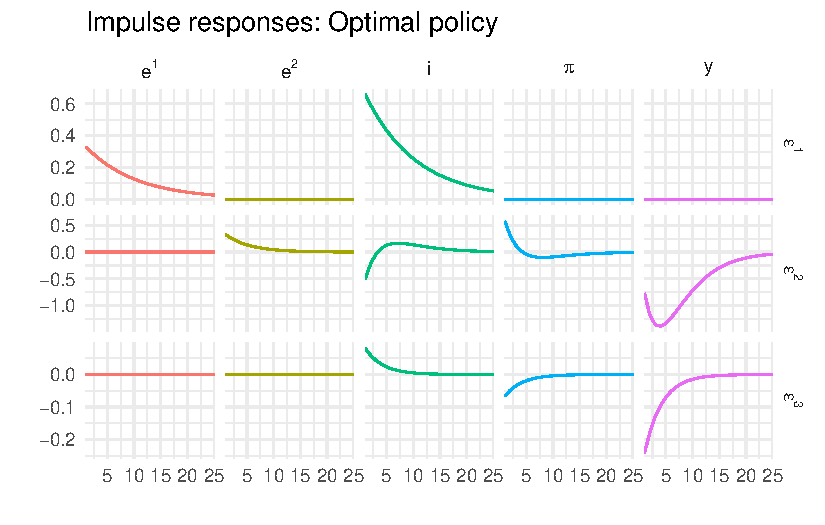
\includegraphics{./BK_files/figure-pdf/unnamed-chunk-26-1.pdf}

}

\end{figure}

\hypertarget{dummy-jumps}{%
\section{Dummy jumps}\label{dummy-jumps}}

But this isn't the only way to get this to work. Effectively what we
just did was create an extra predetermined variable and reorder the
system to give us non-singularity. What if instead of including an
unused \(i_{t-1}\) on the right hand side, we instead include an unused
\(i^e_{t+1}\) on the left hand side? So we swap to having one more jump
variable, one less predetermined one?

Compare the following to the previous model. When we pick out the
interest rate we do so on the right hand side of the matrix equation,
not the left as before.

\begin{Shaded}
\begin{Highlighting}[]
\NormalTok{ns }\OtherTok{\textless{}{-}} \DecValTok{6}      \CommentTok{\# One extra state}
\NormalTok{nf }\OtherTok{\textless{}{-}} \DecValTok{3}      \CommentTok{\# And one extra jump}
\NormalTok{np }\OtherTok{\textless{}{-}}\NormalTok{ ns}\SpecialCharTok{{-}}\NormalTok{nf}
\NormalTok{labels }\OtherTok{\textless{}{-}} \FunctionTok{c}\NormalTok{(}\StringTok{"e\^{}1"}\NormalTok{,}\StringTok{"e\^{}2"}\NormalTok{,}\StringTok{"ylag"}\NormalTok{,}\StringTok{"i"}\NormalTok{,}\StringTok{"y"}\NormalTok{,}\StringTok{"pi"}\NormalTok{) }\CommentTok{\# New variable order}

\NormalTok{E }\OtherTok{\textless{}{-}} \FunctionTok{matrix}\NormalTok{(}\DecValTok{0}\NormalTok{,ns,ns)}
\NormalTok{A }\OtherTok{\textless{}{-}}\NormalTok{ E}
\NormalTok{B }\OtherTok{\textless{}{-}} \FunctionTok{matrix}\NormalTok{(}\DecValTok{0}\NormalTok{,ns,ne)}
\NormalTok{B[}\DecValTok{1}\NormalTok{,}\DecValTok{1}\NormalTok{] }\OtherTok{\textless{}{-}} \DecValTok{1}
\NormalTok{B[}\DecValTok{2}\NormalTok{,}\DecValTok{2}\NormalTok{] }\OtherTok{\textless{}{-}} \DecValTok{1}
\NormalTok{B[}\DecValTok{4}\NormalTok{,}\DecValTok{3}\NormalTok{] }\OtherTok{\textless{}{-}} \SpecialCharTok{{-}}\DecValTok{1}

\FunctionTok{diag}\NormalTok{(E[}\DecValTok{1}\SpecialCharTok{:}\DecValTok{3}\NormalTok{,}\DecValTok{1}\SpecialCharTok{:}\DecValTok{3}\NormalTok{]) }\OtherTok{\textless{}{-}} \DecValTok{1}
\FunctionTok{diag}\NormalTok{(A[}\DecValTok{1}\SpecialCharTok{:}\DecValTok{2}\NormalTok{,}\DecValTok{1}\SpecialCharTok{:}\DecValTok{2}\NormalTok{]) }\OtherTok{\textless{}{-}} \FunctionTok{c}\NormalTok{(rho\_1, rho\_2)}
\NormalTok{A[}\DecValTok{3}\NormalTok{,}\DecValTok{5}\NormalTok{]           }\OtherTok{\textless{}{-}} \DecValTok{1}

\NormalTok{E[}\DecValTok{4}\NormalTok{,}\DecValTok{3}\NormalTok{]           }\OtherTok{\textless{}{-}} \DecValTok{1}
\NormalTok{A[}\DecValTok{4}\NormalTok{,}\FunctionTok{c}\NormalTok{(}\DecValTok{3}\NormalTok{, }\DecValTok{6}\NormalTok{)]     }\OtherTok{\textless{}{-}} \FunctionTok{c}\NormalTok{(}\DecValTok{1}\NormalTok{, }\SpecialCharTok{{-}}\DecValTok{1}\SpecialCharTok{/}\NormalTok{mu)}

\NormalTok{E[}\DecValTok{5}\NormalTok{,}\FunctionTok{c}\NormalTok{(}\DecValTok{1}\NormalTok{, }\DecValTok{5}\NormalTok{, }\DecValTok{6}\NormalTok{)]  }\OtherTok{\textless{}{-}} \FunctionTok{c}\NormalTok{(}\DecValTok{1}\NormalTok{, }\DecValTok{1}\NormalTok{, }\DecValTok{1}\SpecialCharTok{/}\NormalTok{sigma) }\CommentTok{\# One less coefficient}
\NormalTok{A[}\DecValTok{5}\NormalTok{,}\FunctionTok{c}\NormalTok{(}\DecValTok{4}\NormalTok{, }\DecValTok{5}\NormalTok{)]     }\OtherTok{\textless{}{-}} \FunctionTok{c}\NormalTok{(}\DecValTok{1}\SpecialCharTok{/}\NormalTok{sigma, }\DecValTok{1}\NormalTok{)    }\CommentTok{\# One more {-} nothing else changes}

\NormalTok{E[}\DecValTok{6}\NormalTok{,}\FunctionTok{c}\NormalTok{(}\DecValTok{2}\NormalTok{, }\DecValTok{6}\NormalTok{)]     }\OtherTok{\textless{}{-}} \FunctionTok{c}\NormalTok{(}\DecValTok{1}\NormalTok{, beta)}
\NormalTok{A[}\DecValTok{6}\NormalTok{,}\FunctionTok{c}\NormalTok{(}\DecValTok{5}\NormalTok{, }\DecValTok{6}\NormalTok{)]     }\OtherTok{\textless{}{-}} \FunctionTok{c}\NormalTok{(}\SpecialCharTok{{-}}\NormalTok{kappa, }\DecValTok{1}\NormalTok{)}
\end{Highlighting}
\end{Shaded}

This is still a singular model, as we can see from

\begin{Shaded}
\begin{Highlighting}[]
\NormalTok{E}
\end{Highlighting}
\end{Shaded}

\begin{verbatim}
     [,1] [,2] [,3] [,4] [,5] [,6]
[1,]    1    0    0    0    0 0.00
[2,]    0    1    0    0    0 0.00
[3,]    0    0    1    0    0 0.00
[4,]    0    0    1    0    0 0.00
[5,]    1    0    0    0    1 0.50
[6,]    0    1    0    0    0 0.99
\end{verbatim}

with column 4 all zeros. Is \emph{this} model saddle path stable?

\begin{Shaded}
\begin{Highlighting}[]
\NormalTok{e }\OtherTok{\textless{}{-}}\NormalTok{ geigen}\SpecialCharTok{::}\FunctionTok{gevalues}\NormalTok{(geigen}\SpecialCharTok{::}\FunctionTok{gqz}\NormalTok{(A, E, }\AttributeTok{sort=}\StringTok{"S"}\NormalTok{) )}
\NormalTok{e[}\FunctionTok{abs}\NormalTok{(e) }\SpecialCharTok{\textgreater{}} \DecValTok{1}\NormalTok{]}
\end{Highlighting}
\end{Shaded}

\begin{verbatim}
[1]     -Inf 1.378195      Inf
\end{verbatim}

Again, it is with an extra unstable root for the extra jump variable. We
could simplify the solution. As that top left 3 by 3 block, \(E_{11}\),
is the identity matrix and \(E_{12}\) is all zeros this \texttt{Ei} is
always an identity matrix. However, here we simply re-use
\texttt{solveGenBG}

\begin{Shaded}
\begin{Highlighting}[]
\NormalTok{So2 }\OtherTok{\textless{}{-}} \FunctionTok{solveGenBK}\NormalTok{(E,A,B,np)}
\end{Highlighting}
\end{Shaded}

\begin{verbatim}
[1] "Number of unstable roots is 3"
\end{verbatim}

\begin{Shaded}
\begin{Highlighting}[]
\NormalTok{Po2 }\OtherTok{\textless{}{-}}\NormalTok{ So2}\SpecialCharTok{$}\NormalTok{P}
\NormalTok{Qo2 }\OtherTok{\textless{}{-}}\NormalTok{ So2}\SpecialCharTok{$}\NormalTok{Q}
\end{Highlighting}
\end{Shaded}

Now the solved model is

\begin{Shaded}
\begin{Highlighting}[]
\NormalTok{Po2}
\end{Highlighting}
\end{Shaded}

\begin{verbatim}
     [,1]      [,2]       [,3] [,4] [,5] [,6]
[1,]  0.9  0.000000  0.0000000    0    0    0
[2,]  0.0  0.800000  0.0000000    0    0    0
[3,]  0.0 -1.863455  0.7329156    0    0    0
[4,]  1.8 -1.241330 -0.2446879    0    0    0
[5,]  0.0 -1.863455  0.7329156    0    0    0
[6,]  0.0  1.397591  0.2003133    0    0    0
\end{verbatim}

\begin{Shaded}
\begin{Highlighting}[]
\NormalTok{Qo2}
\end{Highlighting}
\end{Shaded}

\begin{verbatim}
     [,1]      [,2]       [,3]
[1,]    1  0.000000  0.0000000
[2,]    0  1.000000  0.0000000
[3,]    0 -2.329318 -0.7329156
[4,]    2 -1.551663  0.2446879
[5,]    0 -2.329318 -0.7329156
[6,]    0  1.746989 -0.2003133
\end{verbatim}

which is actually identical to our previous solution. This is because I
have preserved the order of the solved-out variables, and shows that the
swap from a predetermined to a jump variable is completely arbitrary.

\hypertarget{substituting-out}{%
\section{Substituting out}\label{substituting-out}}

But even this doesn't exhaust the possible re-parametrisations of the
model. We can reduce the number of jump variables to 1 and find the same
solution. There exist formal methods for reducing models (see King and
Watson (2002)) but there is an obvious way to proceed here. From the
targeting rule, it must be that \[
  y^e_{t+1} = y_t - \frac{1}{\mu}\pi^e_{t+1}
\] as the expected shock is zero. This means the IS curve can be
rewritten \[
y_t = y_t - \frac{1}{\mu}\pi^e_{t+1} - \frac{1}{\sigma} \left (i_t - \pi_{t+1}^e \right ) + e_t^1
\] implying \[
i_t =  \left (1 - \frac{\sigma}{\mu} \right )\pi_{t+1}^e + \sigma e_t^1
\] This is the required interest rate consistent with the targeting rule
holding. Now the only jump variable is the inflation rate as we have
eliminated the expected output gap. \[
\begin{aligned}
y_t    &= y_{t-1} -\frac{1}{\mu} \pi_t  + \frac{1}{\mu} \varepsilon^3_t \\
\pi_t  &= \beta \pi_{t+1}^e + \kappa y_t + e_t^2 \\
i_t    &= \left (1 - \frac{\sigma}{\mu} \right ) \pi_{t+1}^e + \sigma e_t^1 \\
e_t^1  &= \rho_1 e_{t-1}^1 + \varepsilon_t^1 \\ 
e_t^2  &= \rho_2 e_{t-1}^2 + \varepsilon_t^2 
\end{aligned}
\]

We can code this

\begin{Shaded}
\begin{Highlighting}[]
\NormalTok{ns }\OtherTok{\textless{}{-}} \DecValTok{5}      \CommentTok{\# Back to 5 states}
\NormalTok{nf }\OtherTok{\textless{}{-}} \DecValTok{1}      \CommentTok{\# Now only one jump}
\NormalTok{np }\OtherTok{\textless{}{-}}\NormalTok{ ns}\SpecialCharTok{{-}}\NormalTok{nf}

\NormalTok{labels }\OtherTok{\textless{}{-}} \FunctionTok{c}\NormalTok{(}\StringTok{"e\^{}1"}\NormalTok{,}\StringTok{"e\^{}2"}\NormalTok{,}\StringTok{"i"}\NormalTok{,}\StringTok{"y"}\NormalTok{,}\StringTok{"pi"}\NormalTok{) }\CommentTok{\# Lose a y}

\NormalTok{E }\OtherTok{\textless{}{-}} \FunctionTok{matrix}\NormalTok{(}\DecValTok{0}\NormalTok{,ns,ns)}
\NormalTok{A }\OtherTok{\textless{}{-}}\NormalTok{ E}
\NormalTok{B }\OtherTok{\textless{}{-}} \FunctionTok{matrix}\NormalTok{(}\DecValTok{0}\NormalTok{,ns,ne)}
\NormalTok{B[}\DecValTok{1}\NormalTok{,}\DecValTok{1}\NormalTok{] }\OtherTok{\textless{}{-}} \DecValTok{1}
\NormalTok{B[}\DecValTok{2}\NormalTok{,}\DecValTok{2}\NormalTok{] }\OtherTok{\textless{}{-}} \DecValTok{1}
\NormalTok{B[}\DecValTok{4}\NormalTok{,}\DecValTok{3}\NormalTok{] }\OtherTok{\textless{}{-}} \SpecialCharTok{{-}}\DecValTok{1}

\FunctionTok{diag}\NormalTok{(E[}\DecValTok{1}\SpecialCharTok{:}\DecValTok{4}\NormalTok{,}\DecValTok{1}\SpecialCharTok{:}\DecValTok{4}\NormalTok{]) }\OtherTok{\textless{}{-}} \DecValTok{1}
\FunctionTok{diag}\NormalTok{(A[}\DecValTok{1}\SpecialCharTok{:}\DecValTok{2}\NormalTok{,}\DecValTok{1}\SpecialCharTok{:}\DecValTok{2}\NormalTok{]) }\OtherTok{\textless{}{-}} \FunctionTok{c}\NormalTok{(rho\_1, rho\_2)}

\NormalTok{E[}\DecValTok{3}\NormalTok{,}\FunctionTok{c}\NormalTok{(}\DecValTok{1}\NormalTok{, }\DecValTok{3}\NormalTok{, }\DecValTok{5}\NormalTok{)]  }\OtherTok{\textless{}{-}} \FunctionTok{c}\NormalTok{(}\SpecialCharTok{{-}}\NormalTok{sigma, }\DecValTok{1}\NormalTok{, sigma}\SpecialCharTok{/}\NormalTok{mu}\DecValTok{{-}1}\NormalTok{)}

\NormalTok{A[}\DecValTok{4}\NormalTok{,}\FunctionTok{c}\NormalTok{(}\DecValTok{4}\NormalTok{,}\DecValTok{5}\NormalTok{)]      }\OtherTok{\textless{}{-}} \FunctionTok{c}\NormalTok{(}\DecValTok{1}\NormalTok{, }\SpecialCharTok{{-}}\DecValTok{1}\SpecialCharTok{/}\NormalTok{mu)}

\NormalTok{E[}\DecValTok{5}\NormalTok{,}\FunctionTok{c}\NormalTok{(}\DecValTok{2}\NormalTok{, }\DecValTok{4}\NormalTok{, }\DecValTok{5}\NormalTok{)]  }\OtherTok{\textless{}{-}} \FunctionTok{c}\NormalTok{(}\DecValTok{1}\NormalTok{, kappa, beta)}
\NormalTok{A[}\DecValTok{5}\NormalTok{,}\DecValTok{5}\NormalTok{]           }\OtherTok{\textless{}{-}} \DecValTok{1}
\end{Highlighting}
\end{Shaded}

and solve it using

\begin{Shaded}
\begin{Highlighting}[]
\NormalTok{Ss }\OtherTok{\textless{}{-}} \FunctionTok{solveGenBK}\NormalTok{(E,A,B,np)}
\end{Highlighting}
\end{Shaded}

\begin{verbatim}
[1] "Number of unstable roots is 1"
\end{verbatim}

\begin{Shaded}
\begin{Highlighting}[]
\NormalTok{Ps }\OtherTok{\textless{}{-}}\NormalTok{ Ss}\SpecialCharTok{$}\NormalTok{P}
\NormalTok{Qs }\OtherTok{\textless{}{-}}\NormalTok{ Ss}\SpecialCharTok{$}\NormalTok{Q}
\end{Highlighting}
\end{Shaded}

Compare the realized of \texttt{Ps}

\begin{Shaded}
\begin{Highlighting}[]
\NormalTok{Ps}
\end{Highlighting}
\end{Shaded}

\begin{verbatim}
     [,1]      [,2] [,3]       [,4] [,5]
[1,]  0.9  0.000000    0  0.0000000    0
[2,]  0.0  0.800000    0  0.0000000    0
[3,]  1.8 -1.241330    0 -0.2446879    0
[4,]  0.0 -1.863455    0  0.7329156    0
[5,]  0.0  1.397591    0  0.2003133    0
\end{verbatim}

with \texttt{Po} above, say. This is the most `efficient' way of
programming the model, in that we have only five states, and indeed the
repeated behavioural equations we had before have disappeared in the
reduced form solution. Just to confirm this, simulating and plotting
this version gives

\begin{Shaded}
\begin{Highlighting}[]
\FunctionTok{response\_plot}\NormalTok{(}\FunctionTok{impulse\_responses}\NormalTok{(Ps,Qs,Omega,labels,T), }\StringTok{"Optimal, substituted out"}\NormalTok{)}
\end{Highlighting}
\end{Shaded}

\begin{figure}[H]

{\centering 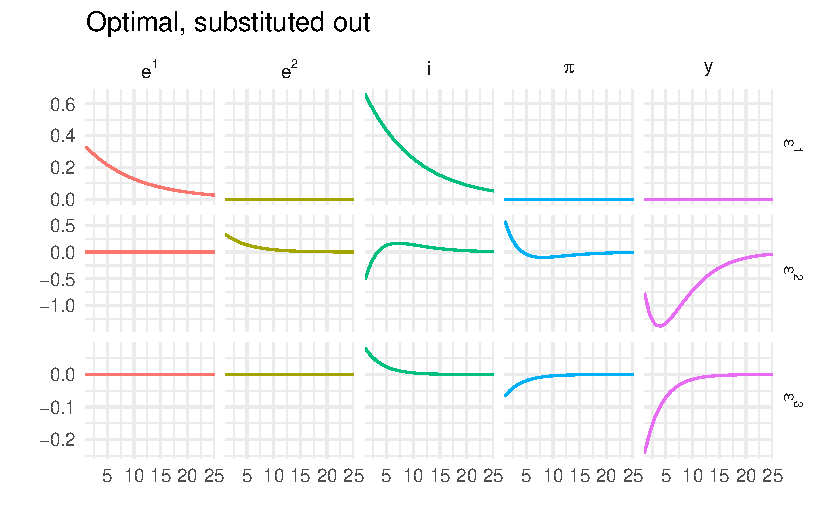
\includegraphics{./BK_files/figure-pdf/unnamed-chunk-35-1.pdf}

}

\end{figure}

which are identical results to those above. But of course \(E\) is now
invertible so we could solve this using the simplest Blanchard-Kahn
variant. Try it!

\hypertarget{bvar-with-dummies}{%
\chapter{BVAR with dummies}\label{bvar-with-dummies}}

\hypertarget{estimating-bvars-using-us-data}{%
\section{Estimating BVARs using US
data}\label{estimating-bvars-using-us-data}}

We will the Fed Funds rate, annual GDP growth and annual CPI inflation
data from FRED, retrieved 2023-05-25. These are:

\begin{figure}

{\centering 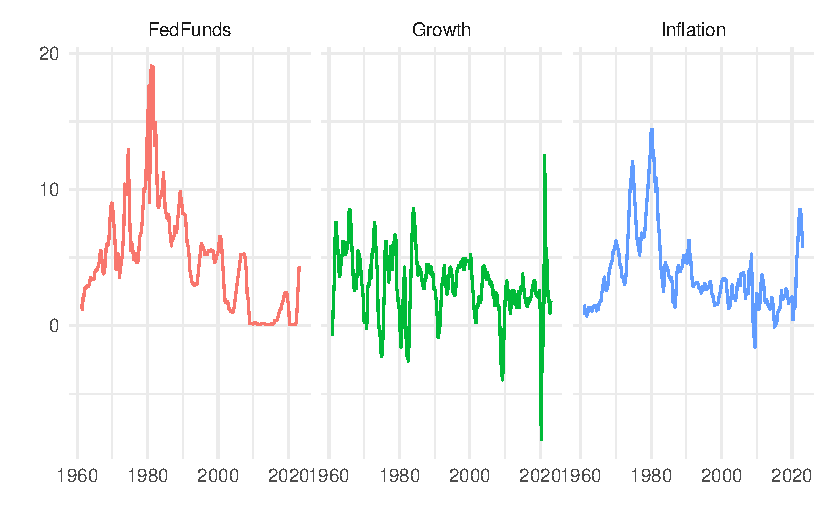
\includegraphics{./BVAR_files/figure-pdf/unnamed-chunk-2-1.pdf}

}

\end{figure}

We will build a variety and two and three variable BVARs. More details
on the data are given below.

\hypertarget{bvars-with-dummy-variable-priors}{%
\section{BVARs with dummy variable
priors}\label{bvars-with-dummy-variable-priors}}

Rather than combine a prior distribution with a likelihood and draw from
the resulting joint posterior distribution there is another convenient
way of parameterizing the problem. We can instead add some `dummy
variables' that have the same properties of the prior so we have a
single modified likelihood that incorporates the prior information. This
approach was most obviously adopted by Banbura, Giannone, and Reichlin
(2010). Further discussion of this can be found in Giannone, Lenza, and
Primiceri (2015). In general this is a version of the Theil and
Goldberger (1961) \textbf{\emph{mixed estimator}} given a Bayesian
interpretation.

\hypertarget{var-model}{%
\subsection{VAR model}\label{var-model}}

Simple bi-variate two-lag VAR model: \[
  \left[\matrix{g_t \cr \pi_t}\right] =
  \left[\matrix{c_1 \cr c_2}\right] +
  \left[\matrix{b_{11} & b_{12} \cr
    b_{21} & b_{22}}\right]
\left[\matrix{g_{t-1} \cr \pi_{t-1} }\right] +
   \left[\matrix{d_{11} & d_{12} \cr
    d_{21} & d_{22}}\right]
\left[\matrix{g_{t-2} \cr \pi_{t-2} }\right] +
  \left[\matrix{\nu_{g,t} \cr \nu_{\pi,t}}\right]
\] \[
  \left[\matrix{\nu_{g,t} \cr \nu_{\pi,t}}\right] \sim N(0, \Sigma)
\]

\hypertarget{bvar-hyperparameters}{%
\section{BVAR hyperparameters}\label{bvar-hyperparameters}}

We will (similarly to the straightforward Minnesota prior) need some
control parameters:

\begin{itemize}
\tightlist
\item
  \(\tau\) controls the overall tightness of the prior for the AR
  coefficients
\item
  \(d\) controls the prior on higher lags;
\item
  \(\lambda\) controls the prior on constants;
\item
  \(\gamma\) controls the prior on the sum of coefficients;
\item
  \(\delta\) controls the cointegration prior;
\end{itemize}

where

\begin{itemize}
\tightlist
\item
  \(\sigma_i\) standard deviation of error terms from individual OLS
  regressions;
\item
  \(\mu_i\) sample means of the data.
\end{itemize}

\hypertarget{first-lag}{%
\subsubsection{First lag}\label{first-lag}}

Now consider the following artificial data for the \textbf{first lag}.
We construct some dummy observations of the dependent and explanatory
variables that look like: \[
  Y_{D,1} = \left[\matrix{\frac{1}{\tau}\sigma_1 & 0 \cr
    0 & \frac{1}{\tau}\sigma_2}\right]
\] and \[
  X_{D,1} = \left [ \matrix{0 & \frac{1}{\tau}\sigma_1 & 0 & 0 & 0\cr
    0 & 0 & \frac{1}{\tau}\sigma_2 & 0 & 0}\right]
\] Intuition: \[
  \left[\matrix{\frac{\sigma_1}{\tau} & 0 \cr
    0 & \frac{\sigma_2}{\tau}}\right] =
  \left[\matrix{0 & \frac{\sigma_1}{\tau} & 0 & 0 & 0\cr
   0 & 0 & \frac{\sigma_2}{\tau} & 0 & 0} \right]
\left[\matrix{c_1    & c_2 \cr
  b_{11} & b_{21} \cr
  b_{12} & b_{22} \cr
  d_{11} & d_{21} \cr
  d_{12} & d_{22}}\right]
+
  \left[\matrix{\xi_{11} & \xi_{12} \cr \xi_{21} & \xi_{22} }\right]
\] Multiplying out we get: \[
  \left[\matrix{\frac{\sigma_1}{\tau} & 0 \cr
    0 & \frac{\sigma_2}{\tau}}\right]
=
  \left[\matrix{\frac{\sigma_1}{\tau}b_{11} &   \frac{\sigma_1}{\tau}b_{21}\cr
  \frac{\sigma_2}{\tau}b_{12} &  \frac{\sigma_2}{\tau}b_{22}} \right]
+
  \left[\matrix{\xi_{11} & \xi_{12} \cr \xi_{21} & \xi_{22} }\right]
\] Concentrating on the first row, notice: \[
  \frac{\sigma_1}{\tau} = \frac{\sigma_1}{\tau}b_{11} + \xi_{11}
\] implying: \[
  b_{11} = 1 - \frac{\tau}{\sigma_1}\xi_{11}
\] so we can write: \[
  b_{11} \sim N\left(1, \frac{\tau^2var(\xi_{11})}{\sigma^2_1}\right)
\] as \(E[b_{11}] = 1 - \frac{\tau}{\sigma_1}E[\xi_{11}] = 1\) and the
variance is easily derived. Similarly: \[
  b_{12} = - \frac{\tau}{\sigma_1}\xi_{12}
\] which is clearly zero in expectation.

\hypertarget{further-priors}{%
\subsection{Further priors}\label{further-priors}}

\hypertarget{higher-lags}{%
\subsubsection{Higher lags}\label{higher-lags}}

Rather than derive the implications we state the rest of the dummy
priors. Consider the following artificial data for the \textbf{second}
lag: \[
Y_{D,2} = \left[\matrix{0 & 0 \cr 0 & 0}\right]
\] and: \[
X_{D,2} = \left [ \matrix{0 & 0 & 0 & \frac{\sigma_1 2^d}{\tau} & 0 \cr
    0 & 0 & 0 & 0 & \frac{\sigma_2 2^d}{\tau} }\right]
\] We can multiply these out and check the properties, in particular we
can verify in the same way as for the first lag that: \[
  b_{ji} \sim N\left(0, \frac{1}{4}\frac{\tau^2var(\xi_{ji})} {2^d\sigma^2_j}\right)
\] for \(j=1,...N\), \(i=1,...l\).

\hypertarget{constant}{%
\subsubsection{Constant}\label{constant}}

Consider the following artificial data for the \textbf{constant}: \[
  Y_{D,3} = \left[\matrix{0 & 0 }\right]
\] \[
  X_{D,3} = \left [ \matrix{\lambda & 0 & 0 & 0 & 0 }\right]
\] so \(\lambda c_1 = \varepsilon_1\) and
\(\lambda c_2 = \varepsilon_2\). As \(\lambda \rightarrow \infty\) the
prior is implemented more tightly.

\hypertarget{covariances}{%
\subsubsection{Covariances}\label{covariances}}

Dummy observations to implement the prior on the error covariance matrix
are: \[
  Y_{D,4} = \left[\matrix{\sigma_1 & 0 \cr 0 & \sigma_2}\right]
\] and \[
  X_{D,4} = \left [ \matrix{0 & 0 & 0 & 0 & 0 \cr
    0 & 0 & 0 & 0 & 0 }\right]
\] with the magnitude of the diagonal elements of \(\Sigma\) controlled
by the scale of the diagonal elements of \(Y_{D,4}\), as larger diagonal
elements implement the prior belief that the variance of \(\nu_1\) and
\(\nu_2\) is larger.

Banbura, Giannone, and Reichlin (2010) stop here, but there are
additional priors that could be added.

\hypertarget{sum-of-coefficients}{%
\subsubsection{Sum of coefficients}\label{sum-of-coefficients}}

We could add a prior that reflects the belief that the \textbf{sum of
coefficients} on `own' lags add up to 1. This is an additional `unit
root'-style prior. Consider: \[
  Y_{D,5} = \left[\matrix{\gamma\mu_1 & 0\cr 0 & \gamma\mu_2}\right]
\] and \[
  X_{D,5} = \left [ \matrix{0 & \gamma\mu_1 & 0 & \gamma\mu_1 & 0\cr
    0 & 0 & \gamma\mu_2 & 0 & \gamma\mu_2}\right]
\] where \(\mu_1\) is the sample mean of \(y_t\) and \(\mu_2\) is the
sample mean of \(x_t\). Note that these dummy observations imply prior
means of the form \(b_{ii} + d_{ii} = 1\) where \(i = 1, 2\) and
\(\gamma\) controls the tightness of the prior. As
\(\gamma \rightarrow \infty\) the prior is implemented more tightly.
Forecast growth rates eventually converge to their sample averages.

\hypertarget{trends}{%
\subsubsection{Trends}\label{trends}}

We can also specify \textbf{common stochastic trend} dummies: \[
  Y_{D,6} = \left[\matrix{\delta\mu_1 & \delta\mu_2 }\right]
\] and \[
  X_{D,6} = \left [ \matrix{\delta & \delta\mu_1 & \delta\mu_2 & \delta\mu_1 & \delta\mu_2 }\right]
\] where this imposes that the coefficients are consistent with limiting
the amount of drift between the predictions at their average values.

\hypertarget{implementation}{%
\subsection{Implementation}\label{implementation}}

The data and the artificial data are now stacked: \[
  Y^* = \left[\matrix{ g_3 & \pi_3 \cr
    \vdots & \vdots \cr
    g_T & \pi_T \cr
    \frac{1}{\tau}\sigma_1 & 0 \cr
    0 & \frac{1}{\tau}\sigma_2\cr
    0 & 0 \cr
    0 & 0 \cr
    0 & 0 \cr
    \sigma_1 & 0 \cr
    0 & \sigma_2 \cr
    \gamma\mu_1 & 0 \cr
    0 & \gamma\mu_2 \cr
    \delta\mu_1 & \delta\mu_2 }\right], \quad
X^* = \left [ \matrix{1 & g_2 & \pi_2 & g_1 & \pi_1 \cr
  \vdots & \vdots & \vdots & \vdots & \vdots \cr
  1 & g_{T-1} & \pi_{T-1} & g_{T-2} & \pi_{T-2} \cr
  0 & \frac{1}{\tau}\sigma_1 & 0 & 0 & 0\cr
  0 & 0 & \frac{1}{\tau}\sigma_2 & 0 & 0\cr
  0 & 0 & 0 & \frac{\sigma_1 2^d}{\tau} & 0 \cr
  0 & 0 & 0 & 0 & \frac{\sigma_2 2^d}{\tau} \cr
  \lambda & 0 & 0 & 0 & 0 \cr
  0 & 0 & 0 & 0 & 0 \cr
  0 & 0 & 0 & 0 & 0 \cr
  0 & \gamma\mu_1 & 0 & \gamma\mu_1 & 0 \cr
  0 & 0 & \gamma\mu_2 & 0 & \gamma\mu_2 \cr
  \delta & \delta\mu_1 & \delta\mu_2 & \delta\mu_1 & \delta\mu_2 }\right]
\] Estimation via Gibbs sampling now proceeds in a very straightforward
way. There is no need to draw for the prior separately.

\hypertarget{examples}{%
\section{Examples}\label{examples}}

First we use quarterly US Growth (FRED series
\href{https://fred.stlouisfed.org/series/A191RO1Q156NBEA}{A191RO1Q156NBEA})
and CPI (FRED series
\href{https://fred.stlouisfed.org/series/CPALTT01USQ661S}{CPALTT01USQ661S})
expressed as the annual inflation rate from 1961-01-01 to 2023-01-01 in
a bi-variate BVAR. The last ten observations are:

\begin{longtable}[]{@{}lrr@{}}
\toprule()
Date & Growth & Inflation \\
\midrule()
\endhead
2020-10-01 & -1.5 & 1.224176 \\
2021-01-01 & 1.2 & 1.905310 \\
2021-04-01 & 12.5 & 4.776278 \\
2021-07-01 & 5.0 & 5.264633 \\
2021-10-01 & 5.7 & 6.765892 \\
2022-01-01 & 3.7 & 8.023109 \\
2022-04-01 & 1.8 & 8.556077 \\
2022-07-01 & 1.9 & 8.284860 \\
2022-10-01 & 0.9 & 7.110821 \\
2023-01-01 & 1.6 & 5.769521 \\
\bottomrule()
\end{longtable}

We specify a VAR with two lags, and use it to forecast 12 periods ahead.
The BVAR are specified using the names above, with only \texttt{tau}
particularly binding in this case. We set the total number of iterations
in each case to 20000 and discard the first half. The parameter
\texttt{nb} is used to set how much back data should appear in a fan
chart.

\begin{Shaded}
\begin{Highlighting}[]
\DocumentationTok{\#\#\#\#\#\#\#\#\#}
\CommentTok{\# Options}
\DocumentationTok{\#\#\#\#\#\#\#\#\#}
\NormalTok{nf }\OtherTok{\textless{}{-}} \DecValTok{12} \CommentTok{\# Max forecast horizon}
\NormalTok{nb }\OtherTok{\textless{}{-}} \DecValTok{21} \CommentTok{\# No. back periods plotted in graphs}
\NormalTok{l  }\OtherTok{\textless{}{-}} \DecValTok{2}  \CommentTok{\# Number of lags in VAR}

\CommentTok{\# specify parameters of the Minnesota{-}type prior}
\NormalTok{tau    }\OtherTok{\textless{}{-}}\NormalTok{ .}\DecValTok{1}   \CommentTok{\# controls prior on own 1st lags (1 makes wibbly)}
\NormalTok{d      }\OtherTok{\textless{}{-}} \DecValTok{1}    \CommentTok{\# decay for higher lags}
\NormalTok{lambda }\OtherTok{\textless{}{-}} \DecValTok{1}    \CommentTok{\# prior for the constant}
\NormalTok{gamma  }\OtherTok{\textless{}{-}} \DecValTok{1}    \CommentTok{\# sum of coefficients unit roots}
\NormalTok{delta  }\OtherTok{\textless{}{-}} \DecValTok{1}    \CommentTok{\# cointegration prior}

\CommentTok{\# Gibbs control}
\NormalTok{reps }\OtherTok{\textless{}{-}} \DecValTok{20000} \CommentTok{\# total numbers of Gibbs iterations}
\NormalTok{burn }\OtherTok{\textless{}{-}} \DecValTok{10000} \CommentTok{\# number of burn{-}in iterations}
\end{Highlighting}
\end{Shaded}

In what follows we vary \texttt{tau} and the lag length to illustrate
their effects. To do this we create the augmented data and then run the
Gibbs sampler, using:

\begin{Shaded}
\begin{Highlighting}[]
\CommentTok{\# Create augmented data}
\NormalTok{Yplus }\OtherTok{\textless{}{-}} \FunctionTok{augmentData}\NormalTok{(Y, l, tau, d, lambda, gamma, delta)}

\CommentTok{\# Run Gibbs sampler}
\NormalTok{out   }\OtherTok{\textless{}{-}} \FunctionTok{Gibbs\_estimate}\NormalTok{(Yplus[[}\DecValTok{1}\NormalTok{]], Yplus[[}\DecValTok{2}\NormalTok{]], reps, burn, }\DecValTok{1}\NormalTok{, nf)}
\end{Highlighting}
\end{Shaded}

where \texttt{Y} contains the data in a dataframe/tibble with the date
in the first column as in the data example above. The code strips out
the date and then uses the remaining \(N\) columns in the BVAR. See the
Code Appendix for the details of the functions.

The output contains any \textbf{\emph{forecast}} draws from the Gibbs
sampler in the third list element from the \texttt{Gibbs\_estimate()}
function. The first two elements are coefficient draws. Two further
functions plots the fan charts using the Gibbs draws:

\begin{Shaded}
\begin{Highlighting}[]
\CommentTok{\# String to put in subtitle}
\NormalTok{controls }\OtherTok{\textless{}{-}} \FunctionTok{paste0}\NormalTok{(}\StringTok{"Lag length "}\NormalTok{, l, }\StringTok{": tau="}\NormalTok{, tau, }\StringTok{", d="}\NormalTok{, d,}
                   \StringTok{", lambda="}\NormalTok{, lambda, }\StringTok{", gamma="}\NormalTok{, gamma, }\StringTok{", delta="}\NormalTok{, delta)}

\CommentTok{\# Plots}
\FunctionTok{fan\_chart}\NormalTok{(Y, out[[}\DecValTok{3}\NormalTok{]], controls, nb)}
\NormalTok{p           }\OtherTok{\textless{}{-}} \FunctionTok{coeff\_plot}\NormalTok{(Y, l, out[[}\DecValTok{1}\NormalTok{]], out[[}\DecValTok{2}\NormalTok{]], }\DecValTok{333}\NormalTok{, controls)}
\NormalTok{pnum        }\OtherTok{\textless{}{-}}\NormalTok{ pnum}\SpecialCharTok{+}\DecValTok{1}
\NormalTok{pce[[pnum]] }\OtherTok{\textless{}{-}}\NormalTok{ p[[}\DecValTok{1}\NormalTok{]]}
\end{Highlighting}
\end{Shaded}

where the string \texttt{controls} is put in the chart subtitle and the
coefficient densities. It can be anything but is a good place to remind
yourself of how you specified the model. Notice we save the coefficient
plots for later use.

\hypertarget{example-1-bvar2-with-tau0.1}{%
\subsubsection{\texorpdfstring{Example 1: BVAR(2) with
\(\tau=0.1\)}{Example 1: BVAR(2) with \textbackslash tau=0.1}}\label{example-1-bvar2-with-tau0.1}}

\begin{figure}

{\centering 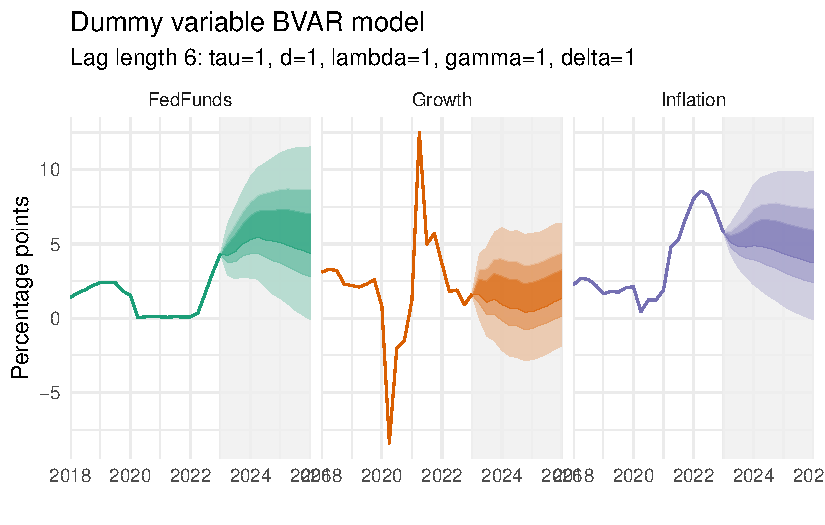
\includegraphics{./BVAR_files/figure-pdf/estim-1.pdf}

}

\end{figure}

\hypertarget{example-2-bvar2-with-tau1}{%
\subsubsection{\texorpdfstring{Example 2: BVAR(2) with
\(\tau=1\)}{Example 2: BVAR(2) with \textbackslash tau=1}}\label{example-2-bvar2-with-tau1}}

\begin{figure}

{\centering 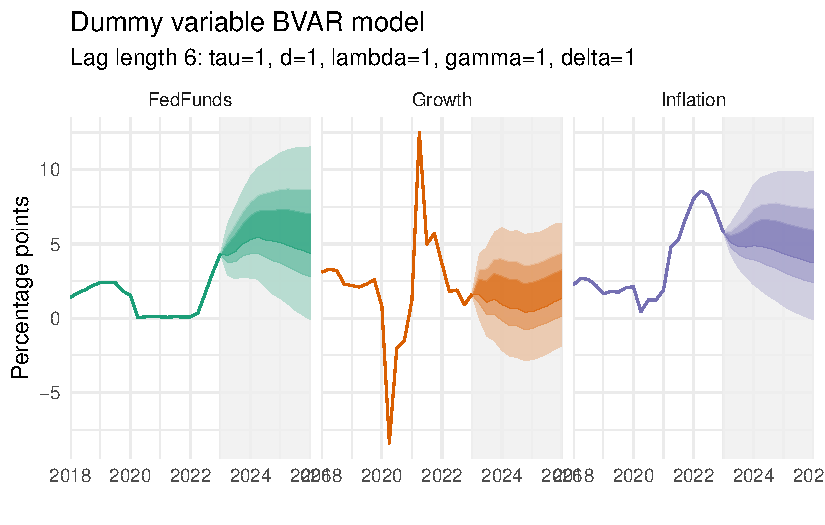
\includegraphics{./BVAR_files/figure-pdf/estim-1.pdf}

}

\end{figure}

\hypertarget{example-3-bvar6-with-tau0.1}{%
\subsubsection{\texorpdfstring{Example 3: BVAR(6) with
\(\tau=0.1\)}{Example 3: BVAR(6) with \textbackslash tau=0.1}}\label{example-3-bvar6-with-tau0.1}}

\begin{figure}

{\centering 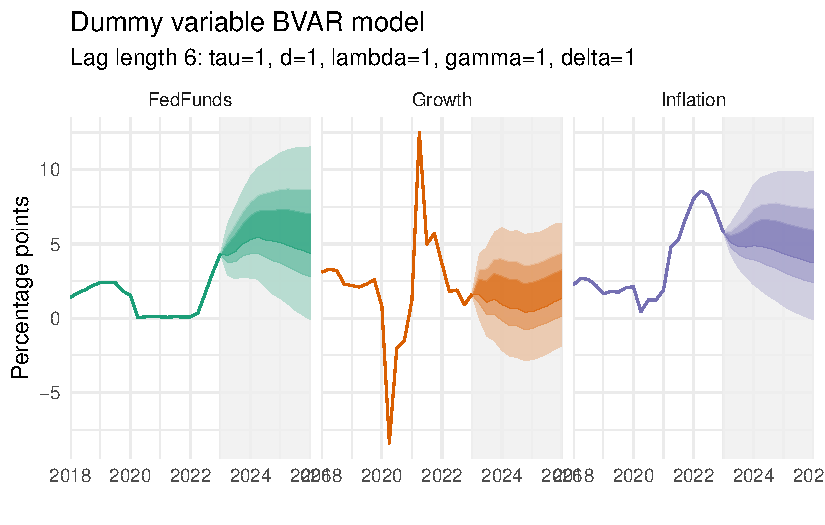
\includegraphics{./BVAR_files/figure-pdf/estim-1.pdf}

}

\end{figure}

\hypertarget{example-4-bvar6-with-tau1}{%
\subsubsection{\texorpdfstring{Example 4: BVAR(6) with
\(\tau=1\)}{Example 4: BVAR(6) with \textbackslash tau=1}}\label{example-4-bvar6-with-tau1}}

\begin{figure}

{\centering 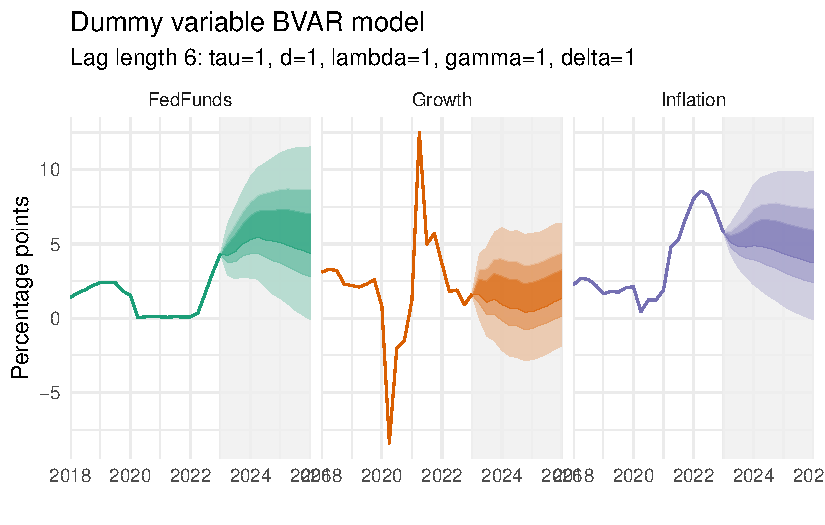
\includegraphics{./BVAR_files/figure-pdf/estim-1.pdf}

}

\end{figure}

\hypertarget{coefficient-estimates}{%
\subsubsection{Coefficient estimates}\label{coefficient-estimates}}

All of these have underlying parameters. Their estimated posterior
densities are:

\begin{figure}

{\centering 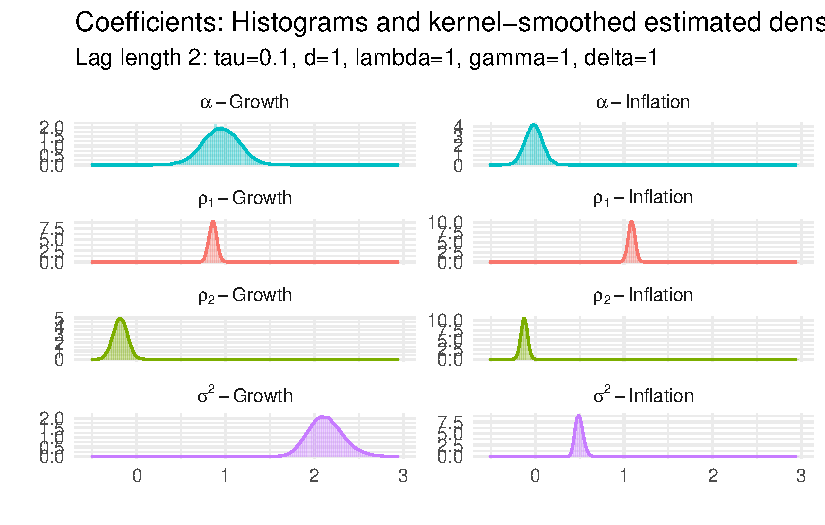
\includegraphics{./BVAR_files/figure-pdf/unnamed-chunk-9-1.pdf}

}

\end{figure}

\begin{figure}

{\centering 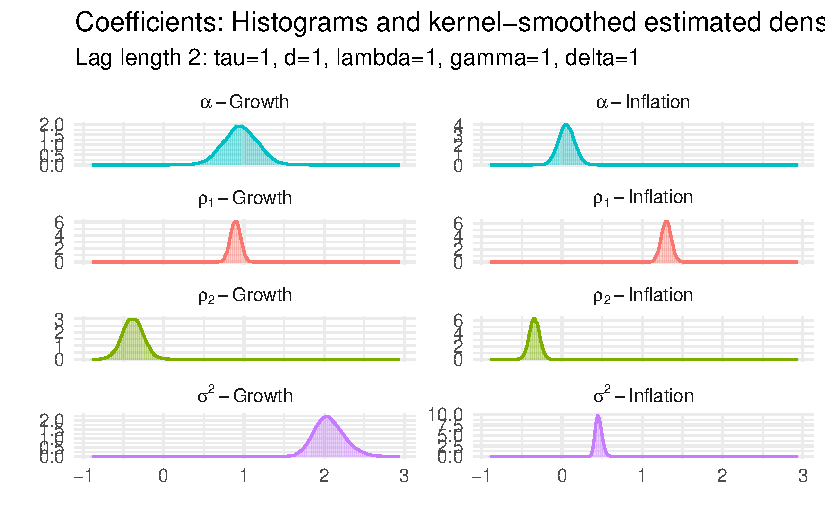
\includegraphics{./BVAR_files/figure-pdf/unnamed-chunk-9-2.pdf}

}

\end{figure}

\begin{figure}

{\centering 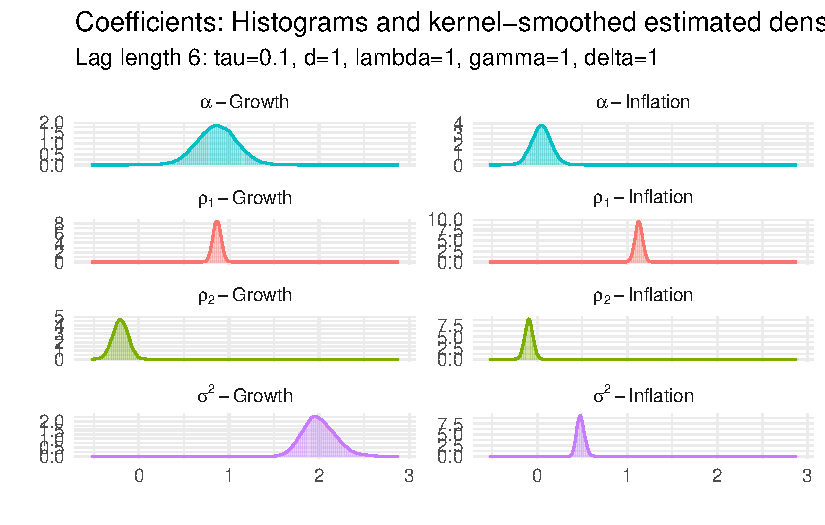
\includegraphics{./BVAR_files/figure-pdf/unnamed-chunk-9-3.pdf}

}

\end{figure}

\begin{figure}

{\centering 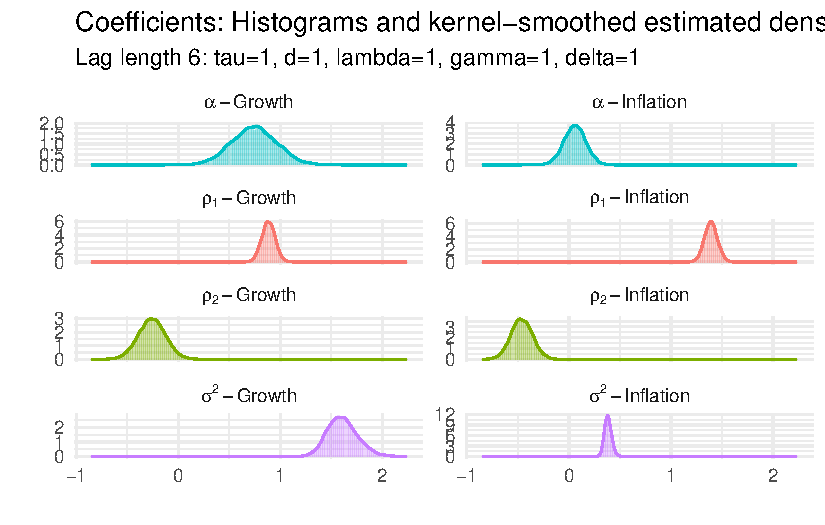
\includegraphics{./BVAR_files/figure-pdf/unnamed-chunk-9-4.pdf}

}

\end{figure}

\hypertarget{tri-variate-bvar}{%
\section{Tri-variate BVAR}\label{tri-variate-bvar}}

Now we add the FedFunds rate (FRED series
\href{https://fred.stlouisfed.org/series/FEDFUNDS}{FEDFUNDS}), so the
last ten periods of the data set is now:

\begin{longtable}[]{@{}lrrr@{}}
\toprule()
Date & Growth & Inflation & FedFunds \\
\midrule()
\endhead
2020-10-01 & -1.5 & 1.224176 & 0.09 \\
2021-01-01 & 1.2 & 1.905310 & 0.09 \\
2021-04-01 & 12.5 & 4.776278 & 0.07 \\
2021-07-01 & 5.0 & 5.264633 & 0.10 \\
2021-10-01 & 5.7 & 6.765892 & 0.08 \\
2022-01-01 & 3.7 & 8.023109 & 0.08 \\
2022-04-01 & 1.8 & 8.556077 & 0.33 \\
2022-07-01 & 1.9 & 8.284860 & 1.68 \\
2022-10-01 & 0.9 & 7.110821 & 3.08 \\
2023-01-01 & 1.6 & 5.769521 & 4.33 \\
\bottomrule()
\end{longtable}

Two more examples follow.

\hypertarget{example-5-bvar4-with-tau.1-3-variables}{%
\subsubsection{\texorpdfstring{Example 5: BVAR(4) with \(\tau=.1\), 3
variables}{Example 5: BVAR(4) with \textbackslash tau=.1, 3 variables}}\label{example-5-bvar4-with-tau.1-3-variables}}

\begin{figure}

{\centering 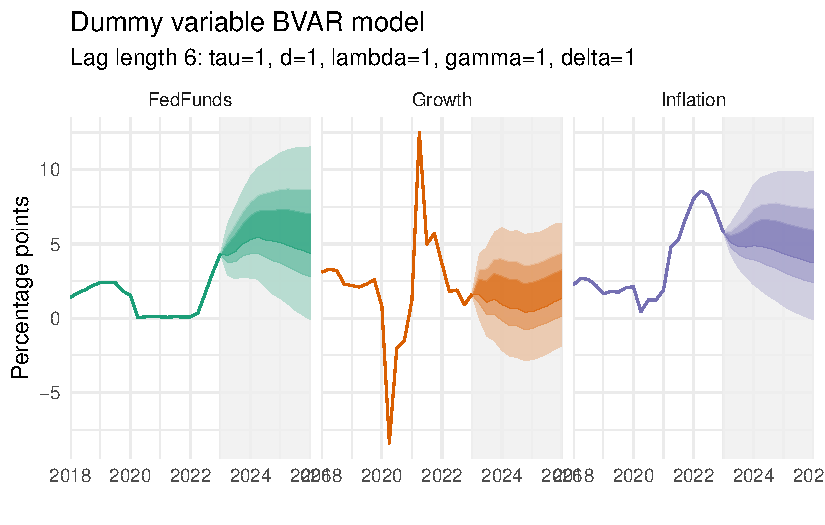
\includegraphics{./BVAR_files/figure-pdf/estim-1.pdf}

}

\end{figure}

\begin{figure}

{\centering 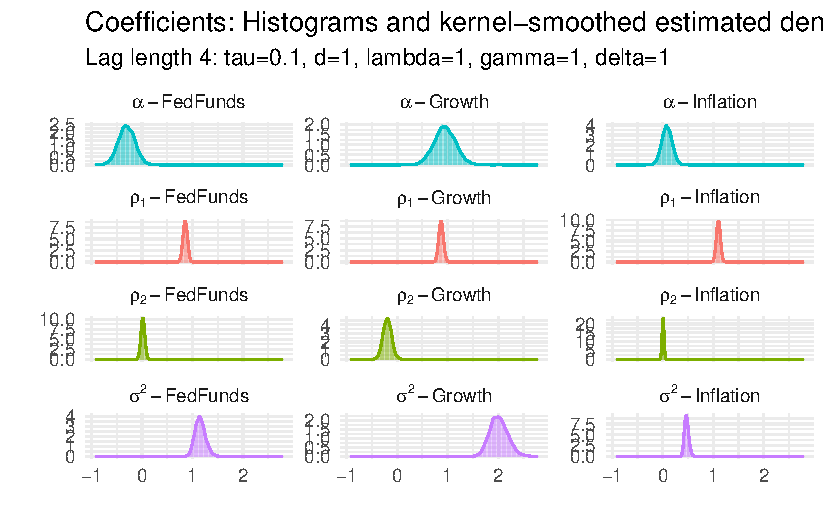
\includegraphics{./BVAR_files/figure-pdf/unnamed-chunk-12-1.pdf}

}

\end{figure}

\hypertarget{example-6-bvar6-with-tau1-3-variables}{%
\subsubsection{\texorpdfstring{Example 6: BVAR(6) with \(\tau=1\), 3
variables}{Example 6: BVAR(6) with \textbackslash tau=1, 3 variables}}\label{example-6-bvar6-with-tau1-3-variables}}

\begin{figure}

{\centering 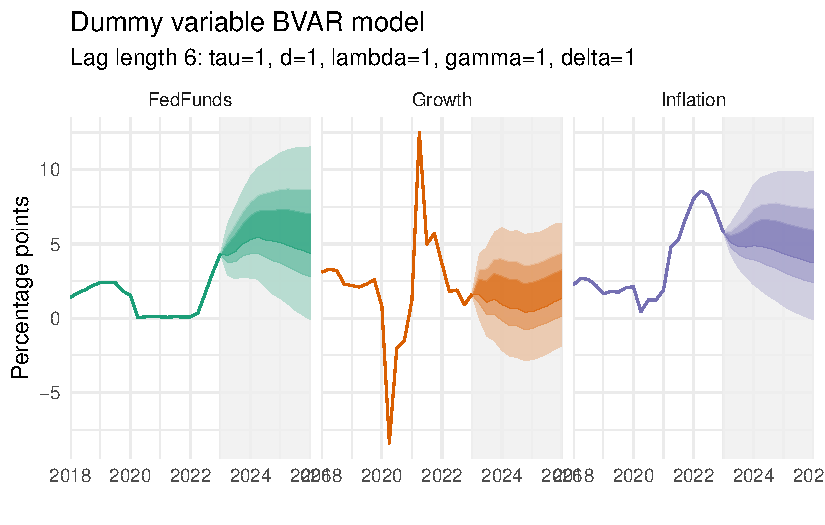
\includegraphics{./BVAR_files/figure-pdf/estim-1.pdf}

}

\end{figure}

\begin{figure}

{\centering 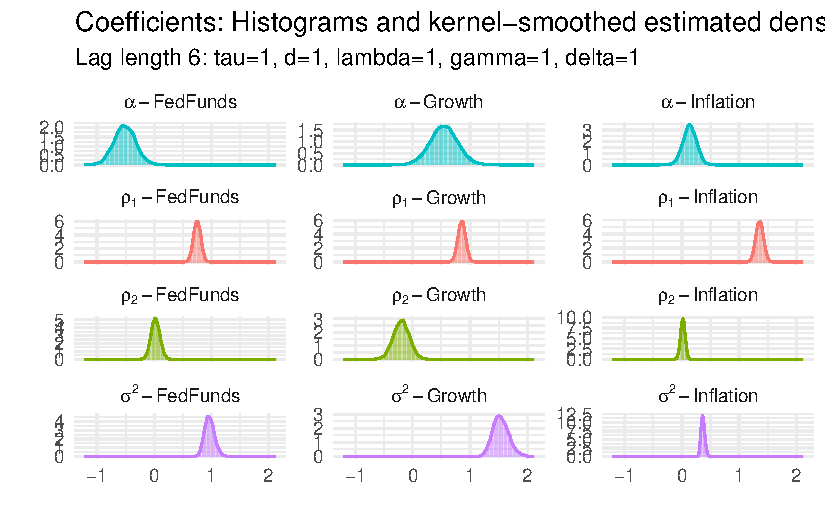
\includegraphics{./BVAR_files/figure-pdf/unnamed-chunk-14-1.pdf}

}

\end{figure}

\hypertarget{code-appendix}{%
\section{Code appendix}\label{code-appendix}}

You can download the program and functions used for the estimates above
from the links below. Put them in the same directory and they should
recreate exactly (within sampling error) the same graphs as above.
Ensure you have all the libraries available that are loaded at the top
of \texttt{BVARdum.R}.

Main program:

Functions:

\part{End matter}

\hypertarget{summary}{%
\chapter{Summary}\label{summary}}

In summary, this book has no content whatsoever\ldots{}

\hypertarget{references}{%
\chapter*{References}\label{references}}
\addcontentsline{toc}{chapter}{References}

\markboth{References}{References}

\hypertarget{refs}{}
\begin{CSLReferences}{1}{0}
\leavevmode\vadjust pre{\hypertarget{ref-BFP}{}}%
Bahaj, Saleem, Angus Foulis, and Gabor Pinter. 2020. {``Home Values and
Firm Behavior.''} \emph{American Economic Review} 110 (7): 2225--70.
\url{https://doi.org/10.1257/aer.20180649}.

\leavevmode\vadjust pre{\hypertarget{ref-Banbura}{}}%
Banbura, M., D. Giannone, and L. Reichlin. 2010. {``Large {B}ayesian
Vector Auto Regressions.''} \emph{Journal of Applied Econometrics} 25
(1): 71--92.

\leavevmode\vadjust pre{\hypertarget{ref-BlakeCE}{}}%
Blake, Andrew P. 2004. {``Analytic Derivatives in Linear Rational
Expectations Models.''} \emph{Computational Economics} 24 (1): 77--96.

\leavevmode\vadjust pre{\hypertarget{ref-Mumtaz_BOOK}{}}%
Blake, Andrew P, and Haroon Mumtaz. 2017. \emph{Applied Bayesian
Econometrics for Central Bankers}. Revised. Technical Books. Centre for
Central Banking Studies, Bank of England.
\url{https://www.bankofengland.co.uk/-/media/boe/files/ccbs/resources/applied-bayesian-econometrics-for-central-bankers-updated-2017.pdf}.

\leavevmode\vadjust pre{\hypertarget{ref-BK80}{}}%
Blanchard, O., and C. Kahn. 1980. {``The Solution of Linear Difference
Models Under Rational Expectations.''} \emph{Econometrica} 48 (5):
1305--11.

\leavevmode\vadjust pre{\hypertarget{ref-HOMLR}{}}%
Boehmke, Brad, and Brandon M. Greenwell. 2019. \emph{Hands-on Machine
Learning with {R}}. The {R} Series. Boca Raton: Chapman \& Hall/CRC.
\url{https://bradleyboehmke.github.io/HOML/}.

\leavevmode\vadjust pre{\hypertarget{ref-Mixtape}{}}%
Cunningham, Scott. 2021. \emph{Causal Inference: The Mixtape}. New Haven
\& London: Yale University Press. \url{https://mixtape.scunning.com/}.

\leavevmode\vadjust pre{\hypertarget{ref-GHV}{}}%
Gelman, Andrew, Jennifer Hill, and Aki Vehtari. 2019. \emph{Regression
and Other Stories}. Cambridge: Cambridge University Press.
\url{http://www.stat.columbia.edu/~gelman/regression}.

\leavevmode\vadjust pre{\hypertarget{ref-PriorsVAR}{}}%
Giannone, Domenico, Michele Lenza, and Giorgio E. Primiceri. 2015.
{``{Prior Selection for Vector Autoregressions}.''} \emph{The Review of
Economics and Statistics} 97 (2): 436--51.

\leavevmode\vadjust pre{\hypertarget{ref-ESL}{}}%
Hastie, Trevor, Robert Tibshirani, and Jerome Friedman. 2009. \emph{The
Elements of Statistical Learning: Data Mining, Inference, and
Prediction}. 2nd ed. New York, NY: Springer.
\url{https://web.stanford.edu/~hastie/ElemStatLearn/}.

\leavevmode\vadjust pre{\hypertarget{ref-SuperText}{}}%
Hvitfeldt, Emil, and Julia Silge. 2021. \emph{Supervised Machine
Learning for Text Analysis in {R}}. Chapman \& Hall: CRC Press.
\url{https://smltar.com/}.

\leavevmode\vadjust pre{\hypertarget{ref-ITSL}{}}%
James, Gareth, Daniela Witten, Trevor Hastie, and Robert Tibshirani.
2021. \emph{An Introduction to Statistical Learning: With Applications
in {R}}. 2nd ed. Springer Texts in Statistics. New York, NY: Springer.
\url{https://www.statlearning.com/}.

\leavevmode\vadjust pre{\hypertarget{ref-KW2002}{}}%
King, Robert G., and Mark W. Watson. 2002. {``System Reduction and
Solution Algorithms for Singular Linear Difference Systems Under
Rational Expectations.''} \emph{Computational Economics} 20 (1--2):
57--86.

\leavevmode\vadjust pre{\hypertarget{ref-Klein}{}}%
Klein, Paul. 2000. {``Using the Generalized {S}chur Form to Solve a
Multivariate Linear Rational Expectations Model.''} \emph{Journal of
Economic Dynamics and Control} 24 (10): 1405--23.

\leavevmode\vadjust pre{\hypertarget{ref-Geocomputation}{}}%
Lovelace, Robin, Jakub Nowosad, and Jannes Muenchow. 2019.
\emph{Geocomputation with {R}}. 1st ed. The {R} Series. Boca Raton:
Chapman \& Hall/CRC. \url{https://geocompr.robinlovelace.net/}.

\leavevmode\vadjust pre{\hypertarget{ref-McElreath}{}}%
McElreath, Richard. 2020. \emph{Statistical Rethinking: A Bayesian
Course with Examples in {R} and Stan}. 2nd ed. Abingdon, Oxfordshire:
CRC Press. \url{https://github.com/rmcelreath/rethinking}.

\leavevmode\vadjust pre{\hypertarget{ref-Pappas}{}}%
Pappas, T., A. J. Laub, and N. R. Sandell. 1980. {``On the Numerical
Solution of the Discrete-Time Algebraic Riccati Equation.''} \emph{IEEE
Transaction on Automatic Control} AC-25.4: 631--41.

\leavevmode\vadjust pre{\hypertarget{ref-Primer}{}}%
Pearl, Judea, Madelyn Glymour, and Nicholas P. Jewell. 2016.
\emph{Causal Inference in Statistics: A Primer}. Chichester: John Wiley
\& Sons. \url{http://bayes.cs.ucla.edu/PRIMER/}.

\leavevmode\vadjust pre{\hypertarget{ref-Silge}{}}%
Silge, Julia, and David Robinson. 2017. \emph{Text Mining with {R}: A
{T}idy Approach}. O'Reilly. \url{https://www.tidytextmining.com/}.

\leavevmode\vadjust pre{\hypertarget{ref-Taddy}{}}%
Taddy, Matt. 2019. \emph{Business Data Science: Combining Machine
Learning and Economics to Optimize, Automate, and Accelerate Business
Decisions}. New York, NY: McGraw-Hill Education.
\url{https://github.com/TaddyLab/BDS}.

\leavevmode\vadjust pre{\hypertarget{ref-Theil}{}}%
Theil, Henri, and Arthur S. Goldberger. 1961. {``On Pure and Mixed
Statistical Estimation in Economics.''} \emph{International Economic
Review} 2: 317--32.

\leavevmode\vadjust pre{\hypertarget{ref-Vaughan}{}}%
Vaughan, D. R. 1970. {``A Non Recursive Algorithm Solution for the
Discrete Riccati Equation.''} \emph{IEEE Transactions on Automatic
Control} AC-15.5: 597--99.

\end{CSLReferences}


\backmatter

\end{document}
